% для компиляции в lualatex!!
\documentclass[12pt, a4paper]{article}
\usepackage[english,russian]{babel}
\usepackage[warn]{mathtext}
\usepackage{natbib} %затекстовые ссылки в виде (автор, год)
%\usepackage[T2A]{fontenc}
%\usepackage[utf8]{inputenc}

\usepackage{xecyr} % Продукт Вашего покорного слуги ;)

\setmainfont{DejaVu Serif}

\usepackage{color}
\usepackage{amssymb,amsmath}
\usepackage{graphicx}
\usepackage{multicol}

\textheight=24cm           % высота текста
\textwidth=16cm            % ширина текста
\oddsidemargin=0pt         % отступ от левого края
\topmargin=-1.5cm          % отступ от верхнего края
\parindent=24pt            % абзацный отступ
\parskip=0pt               % интервал между абзацами
\tolerance=2000            % терпимость к "жидким" строкам
\flushbottom               % выравнивание высоты страниц
%\def\baselinestretch{1.5} % печать с большим интервалом

\title{Динамика литоральных поселений {\it Macoma balthica} в вершине Кандалакшского залива Белого моря.}
\author{С.~А.~Назарова \thanks{e-mail:~sophia.nazarova@gmail.com}, Д.~А.~Аристов, А.~В.~Полоскин}
%\date{}

\begin{document}

\maketitle

\section{Введение}
Супер-важность макомы...

Широко-распространенный вид. 
Модельный объект.
Пищевой объект для камбалы и кого еще?
Важно для заповедника...
Писать ли что это заказной мониторинг от заповедника?..

Цели...
Задачи...

\section{Материал и методика}
Материал для данной работы был собран в ходе экспедиций Группы исследований прибрежных сообществ Лаборатории экологии морского бентоса (гидробиологии) СПбГДТЮ в акватории Кандалакшского государсвтенного заповедника и граничащей с ним зоне. 
Мониторинг плотных поселений {\it Macoma balthica} проводили на 6 участках литорали (рис. \ref{ris:map_Kandalaksha}).
Сборы проводили с 1992 по 2012 год ежегодно в период с 15 июля по 10 августа.\textcolor{red}{какие реально даты?}

Структура материала представлена в таблице \ref{tab:material_Kandalaksha}.
\begin{table}
\begin{tabular}{|*{5}{p{0.2\textwidth}|}} \hline
участок & годы наблюдения & обследованные горизонты литорали & количество проб в однократной съемке & площадь пробоотборника  \\ \hline
о. Горелый Лувеньгских шхер & 1992 -- 2012 & ВГЛ, СГЛ, НГЛ & 1-3 & 1/30, 1/10 \\ \hline
Материковая литораль в районе пос. Лувеньга & 1992-2000, 2002, 2004 & ВГЛ, СГЛ, НГЛ & 12-20 & 1/30 \\ \hline
Эстуарий р. Лувеньги & 1992 -- 2012 & СГЛ & 3 & 1/10 \\ \hline
Литораль Западной Ряшковой салмы о. Ряшкова & 1994 -- 2012 & СГЛ & 2 & 1/10 \\ \hline
Южная губа о. Ряшкова & 2001 -- 2012 & НГЛ & 9-16 & 1/30 \\ \hline
о. Ломнишный & 2007 -- 2012 & НГЛ & 5-10 & 1/30  \\ \hline
\end{tabular}
\caption{Структура использованного в работе материала}
\label{tab:material_Kandalaksha}
\end{table}

На каждом исследованном участке отбирали 3 --- 25 проб площадью 1/30 --- 1/10 м$^2$, которые затем промывали на сите с диаметром ячеи 0,5 -- 1 мм. 
В пробах учитывали всех особей {\it Macoma balthica}, у которых в дальнейшем измеряли максимальный линейный размер (длину) с точностью 0,1 мм. 
Для определения биомассы моллюсков взвешивали на электронных весах с точностью до 1 мг. Для серий проб, где не проводили взвешивание моллюсков, биомассу определяли рассчетным методом с использованием аллометриеской зависимости сырой массы маком от длины их раковины \citep{Maximovich_et_al_1993}.
В дальнейшем рассчитывали показатели средней численности маком на квадратный метр (плотность поселения) и размерно-частотное распределение особоей.
Для построения размерно-частотного распределения шаг размерного класса составлял 1 мм.


В дальнейшем при анализе мы работали с особями с длиной раковины более 1,0 мм по двум причинам. 
Во-первых, для того чтобы сделать сравнимыми результаты с разных участков, где пробы промывались на ситах с разным диаметром ячеи. 
Во-вторых, пробы отбирали в середине лета, то есть к этому моменту молодь этого года частично осела, то есть оценка численности данной группы будет некорректна.
Мы считаем корректной такую редукцию материала, поскольку для Белого моря показано, что усешность пополнения поселений молодью в первую очередь зависит от выживаемости спата зимой (\textcolor{red}{тут ссылка на каких-то Максимовича-Герасимову. 2004 - БиНИИ? или 2012 - Hydrobiology}).





 
%методика из Назаровой-Полоскина
%Материал собран в августе 1992 - 2003 гг. Изучено три литоральных поселения маком: в Илистой губе острова Горелого (участок 1), в эстуарии реки Лувеньги (участок 2) и на материковой литорали к югу от поселка Лувеньга (участок 3). Сборы проведены пробоотборником площадью захвата 1/30 м2. Разовая выборка составляла от 9 до 25 проб с участка. Грунт выбирался до глубины 5 см и промывался на сите с диаметром ячеи 0.5мм.  Всех особей  M. balthica измеряли с точностью 0.1 мм. В каждый момент наблюдений определяли размерную структуру и плотность поселения маком. 



% методика из Аристова
%Оба участка закрыты от волнового воздейст-
%вия. Литораль в районе исследований представляет собой песчаный пляж с примесью
%ила с вкраплениями крупных валунов. Спуск в сублитораль пологий, отчетливо вы-
%раженный пояс фукоидов отсутствует. Население представлено типичными формами,
%такими как Arenicola marina, Macoma balthica, Mya arenaria, Hydrobia ulvae, Microspio sp.
%и др. (Д. А. Аристов, неопубликованные данные).
%В обеих точках производили сборы по следующей методике: в районе нуля глубин
%во время отлива в пределах участков случайным образом выбирали и обследовали не-
%сколько площадок. Поскольку радиусы индивидуальной активности A. islandica и пред-
%полагаемых жертв (двустворчатых моллюсков) существенно различаются, в пределах
%каждой площадки брали пару проб методом вложенных рамок. Первую пробу из пары
%(1/4 м2) брали для учета A. islandica. Грунт из пробы тщательно перебирали вручную,
%всех найденных представителей сем. Naticidae подсчитывали и определяли их видовую
%принадлежность. Вторая проба (1/30 м2) была взята для учета потенциальных жертв —
%двустворчатых моллюсков. Грунт из нее промывали на сите с диаметром ячеи 1 мм,
%а затем остаток разбирали в фотографической кювете с белым дном. Из грунта соби

\section{Результаты}
\subsection{Динамика обилия {\it M.~balthica}}


\newpage
\begin{figure}[h]

\begin{minipage}[b]{.46\linewidth}
%Фигурка в первом ряду слева размер отведенный под весь этот объект -- 0.46 от ширины строки
%Параметр [b] означает, что выравнивание этих министраниц будет по нижнему краю
\begin{center}
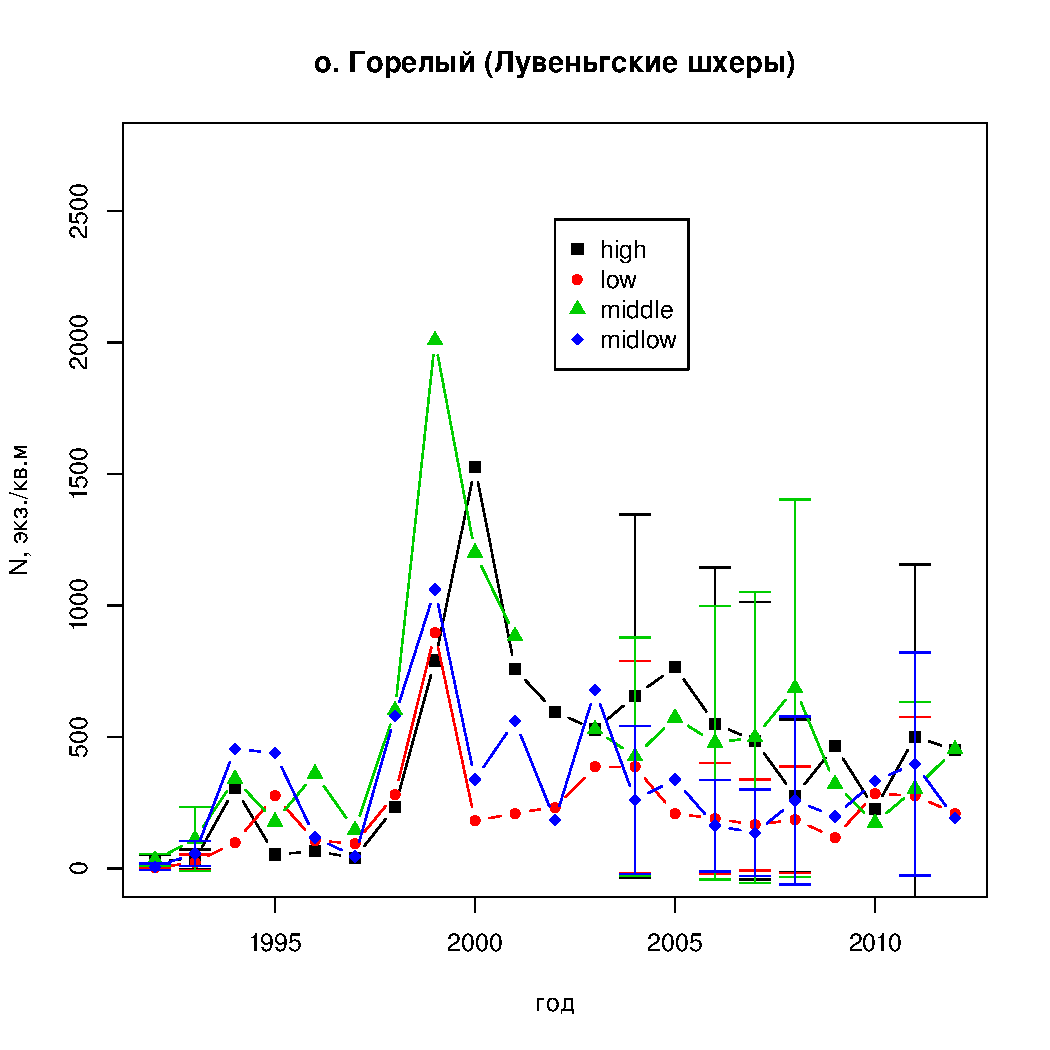
\includegraphics[width=65mm]{../White_Sea/Luvenga_Goreliy/N2_dynamic.pdf}
\end{center}
\end{minipage}
%
\hfil %Это пружинка отодвигающая рисунки друг от друга
%
\begin{minipage}[b]{.46\linewidth}
%Следующий рисунок - первый ряд справа %DUNGEON S_4 \ AB
\begin{center}
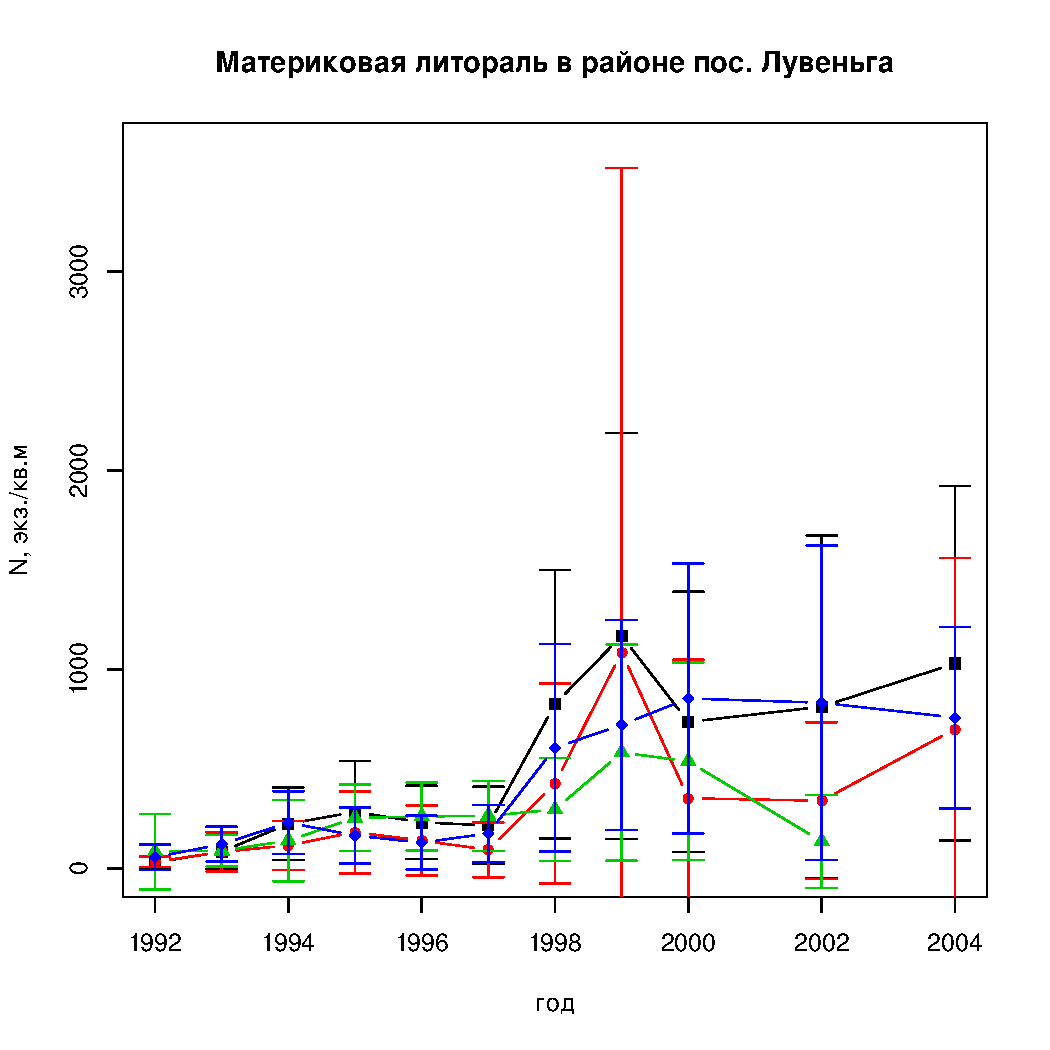
\includegraphics[width=65mm]{../White_Sea//Luvenga_II_razrez/N2_dynamic.pdf}
\end{center}
\end{minipage}

%\smallskip


\begin{minipage}[b]{.46\linewidth}
%Фигурка в первом ряду слева размер отведенный под весь этот объект -- 0.46 от ширины строки
%Параметр [b] означает, что выравнивание этих министраниц будет по нижнему краю
\begin{center}
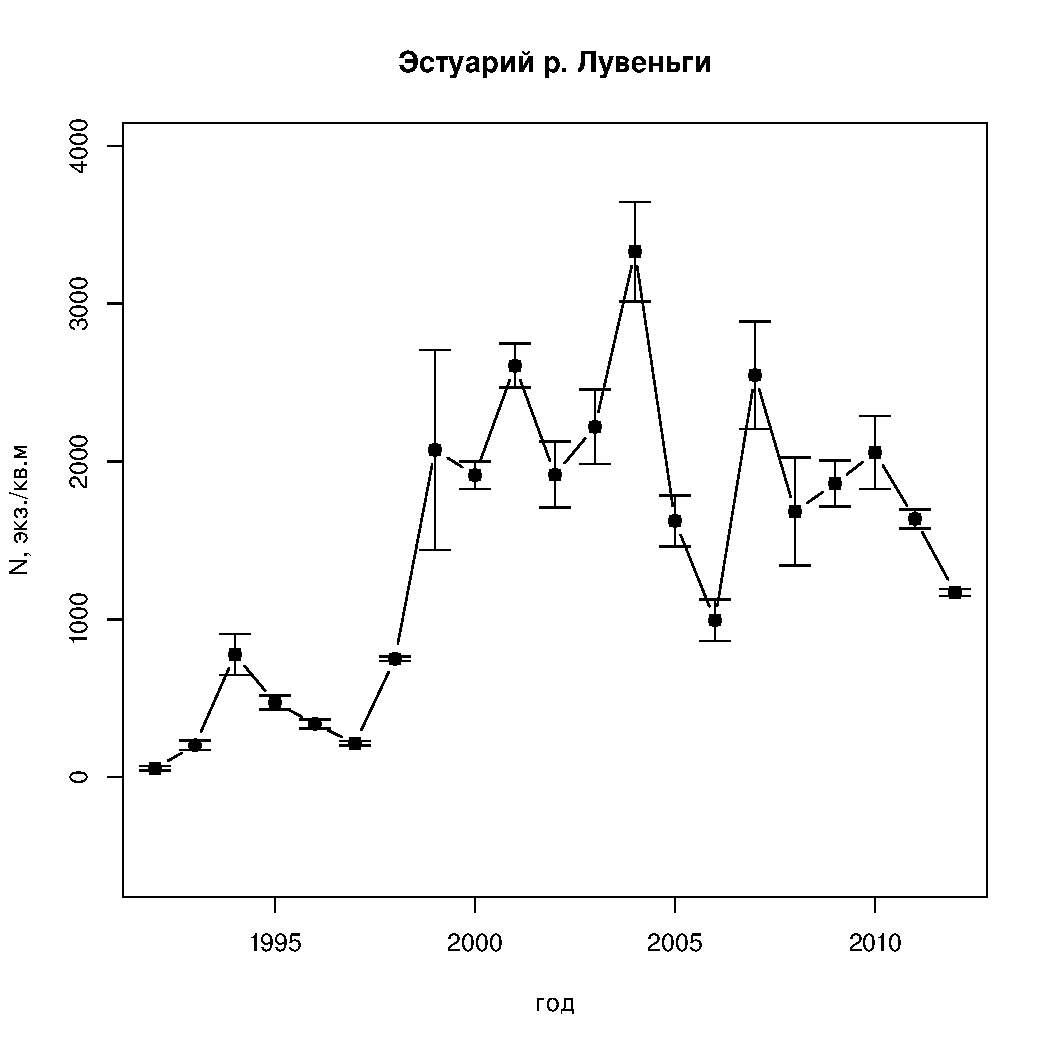
\includegraphics[width=65mm]{../White_Sea/Estuatiy_Luvenga/N2_dynamic.pdf}
\end{center}
\end{minipage}
%
\hfil %Это пружинка отодвигающая рисунки друг от друга
%
\begin{minipage}[b]{.46\linewidth}
%Следующий рисунок - первый ряд справа %DUNGEON S_4 \ AB
\begin{center}
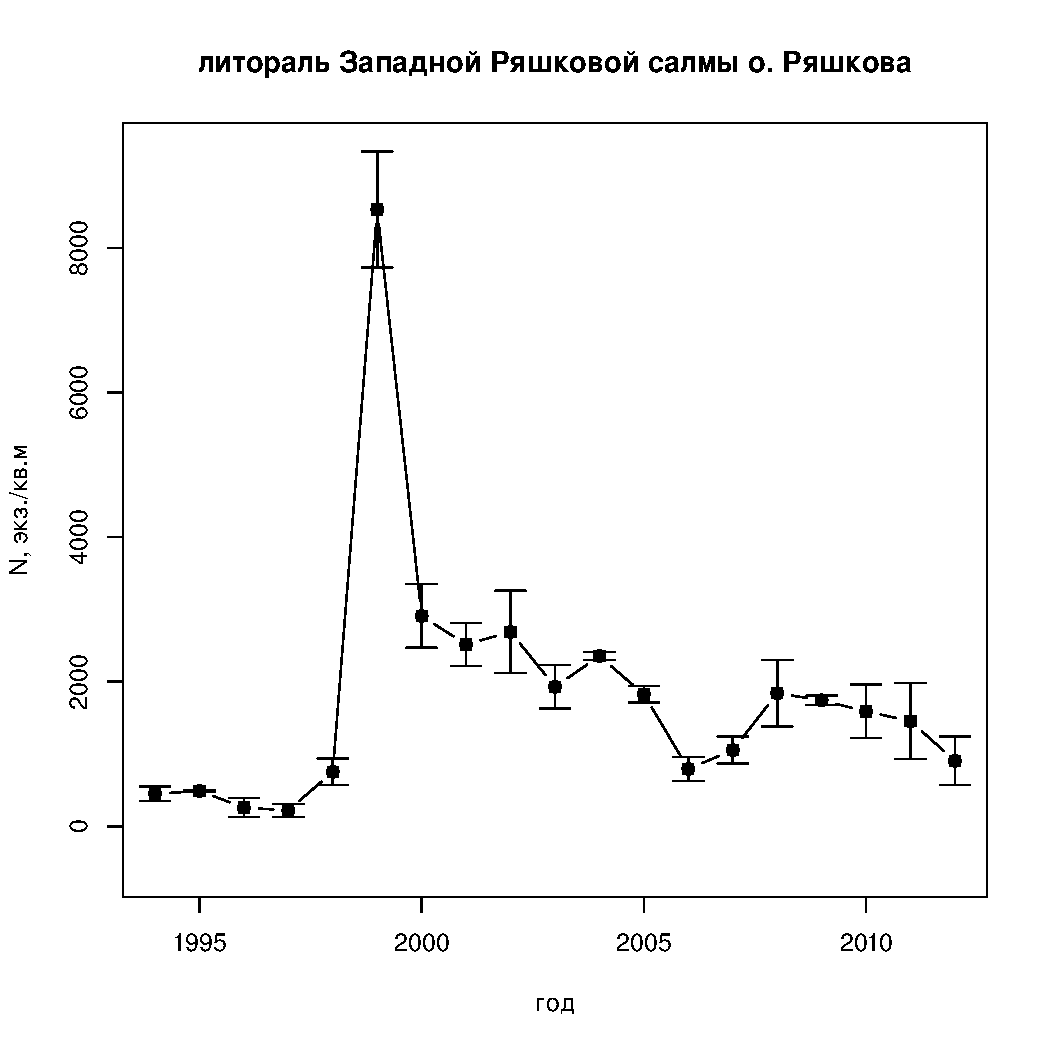
\includegraphics[width=65mm]{../White_Sea/Ryashkov_ZRS/N2_dynamic.pdf}
\end{center}
\end{minipage}

%\smallskip

\begin{minipage}[b]{.46\linewidth}
%Фигурка в первом ряду слева размер отведенный под весь этот объект -- 0.46 от ширины строки
%Параметр [b] означает, что выравнивание этих министраниц будет по нижнему краю
\begin{center}
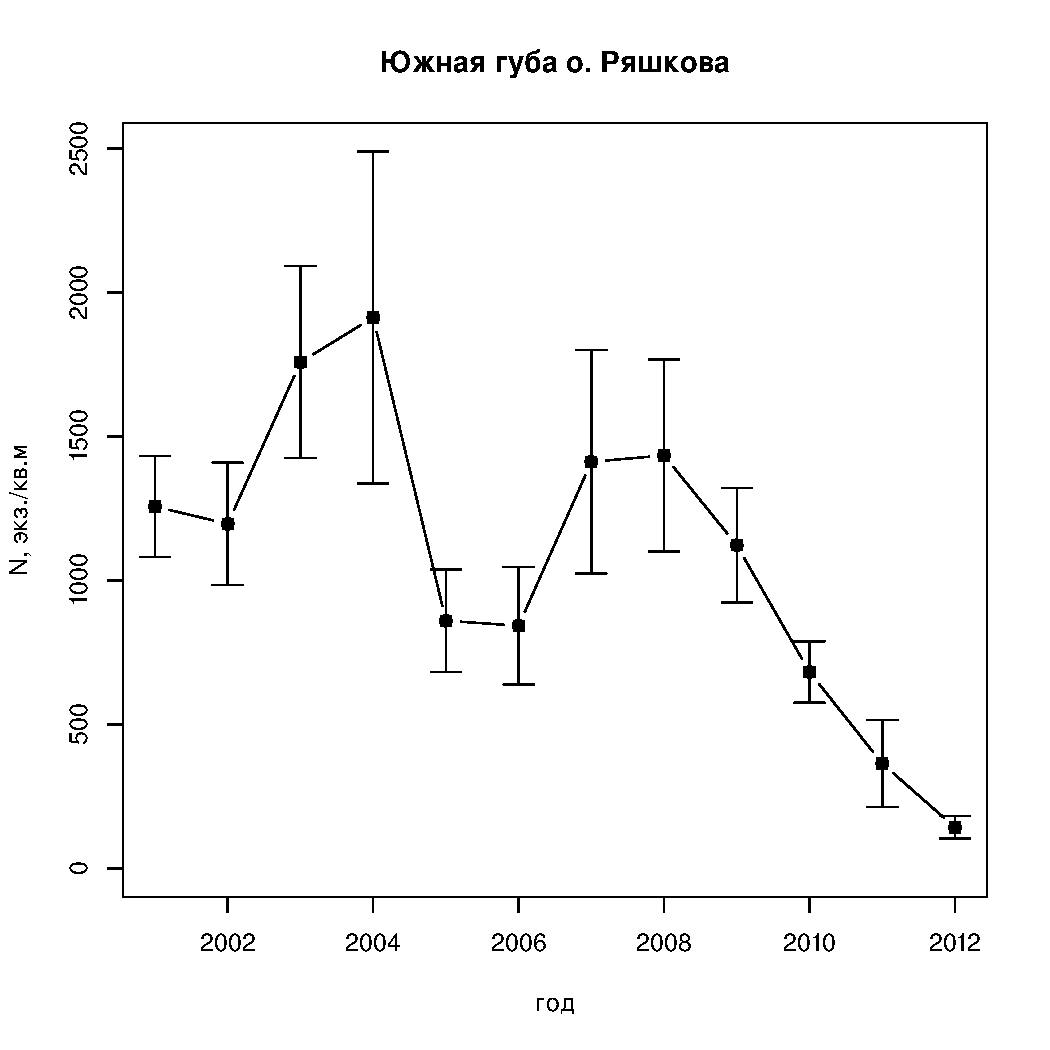
\includegraphics[width=65mm]{../White_Sea/Ryashkov_YuG/N2_dynamic.pdf}
\end{center}
\end{minipage}
%
\hfil %Это пружинка отодвигающая рисунки друг от друга
%
\begin{minipage}[b]{.46\linewidth}
%Следующий рисунок - первый ряд справа %DUNGEON S_4 \ AB
\begin{center}
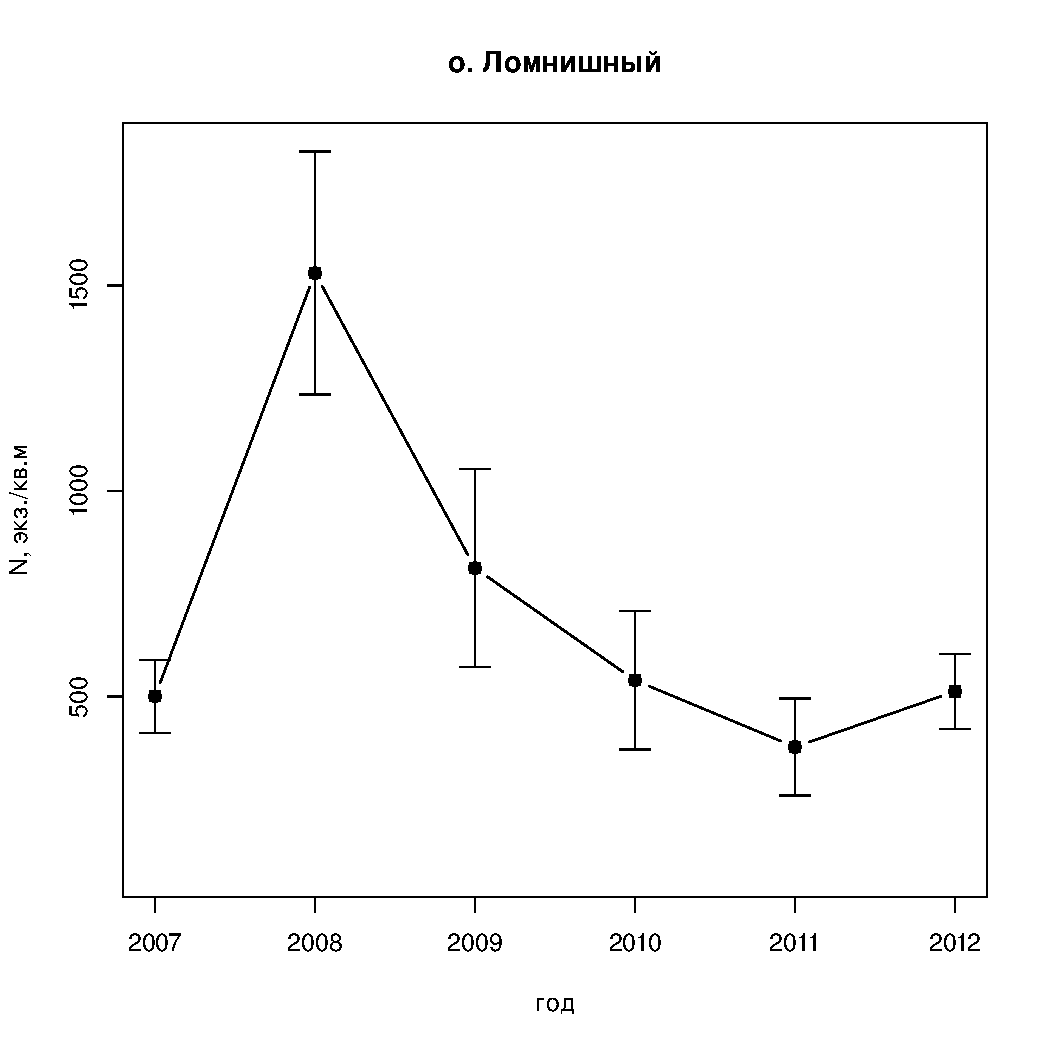
\includegraphics[width=65mm]{../White_Sea/Lomnishniy/N2_dynamic.pdf}
\end{center}
\end{minipage}

%\smallskip


\caption{Динамика численности {\it Macoma balthica} в поселениях вершины Кандалакшского залива}
\label{ris:dynamic_Kandalaksha_all2}
\end{figure}


		\subsection{Размерная структура {\it M.~balthica}}
	\subsubsection{Эстуарий р.~Лувеньги.}



%Эстуарий Лувеньги


\begin{figure}[h]

\begin{multicols}{3}
\hfill
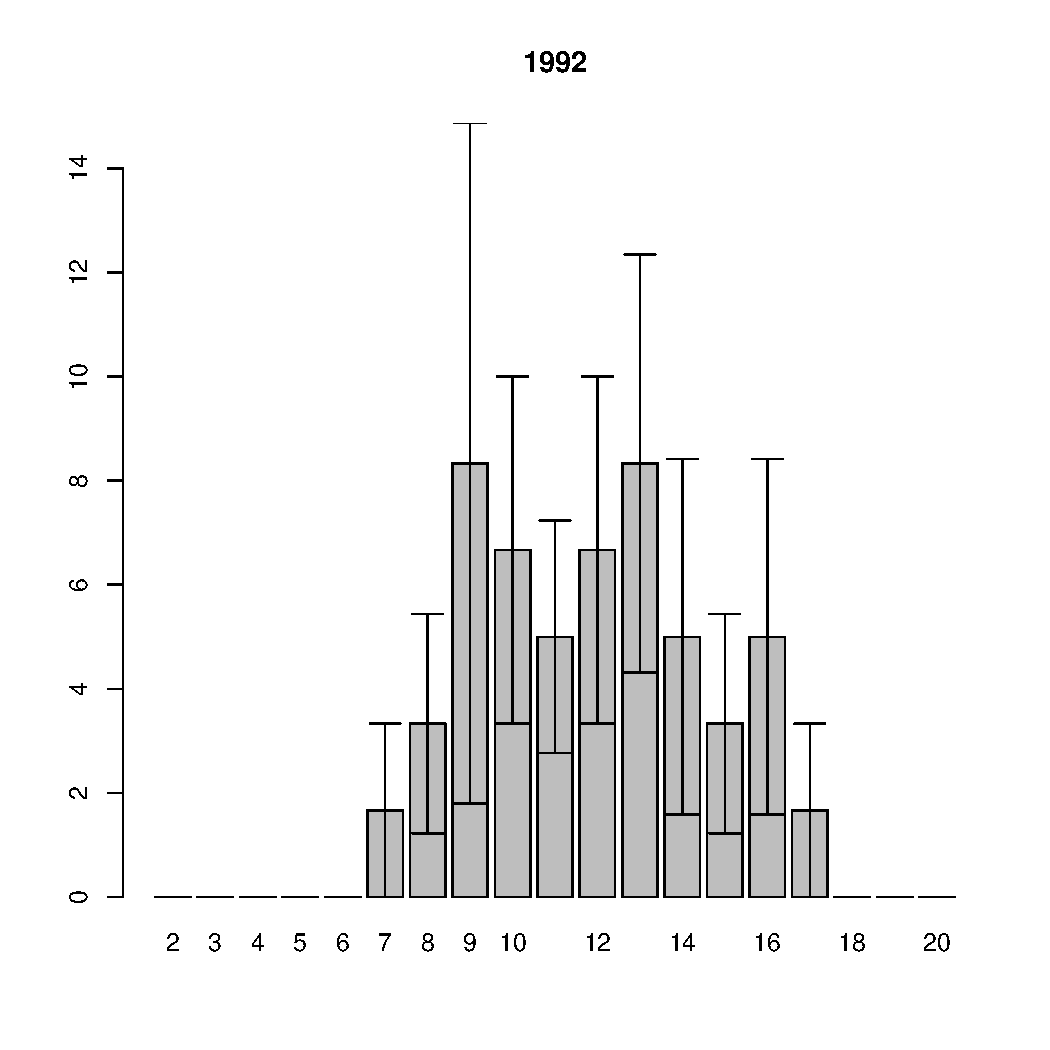
\includegraphics[width=65mm]{../White_Sea/Estuatiy_Luvenga/sizestr2_1992_.pdf}
\hfill
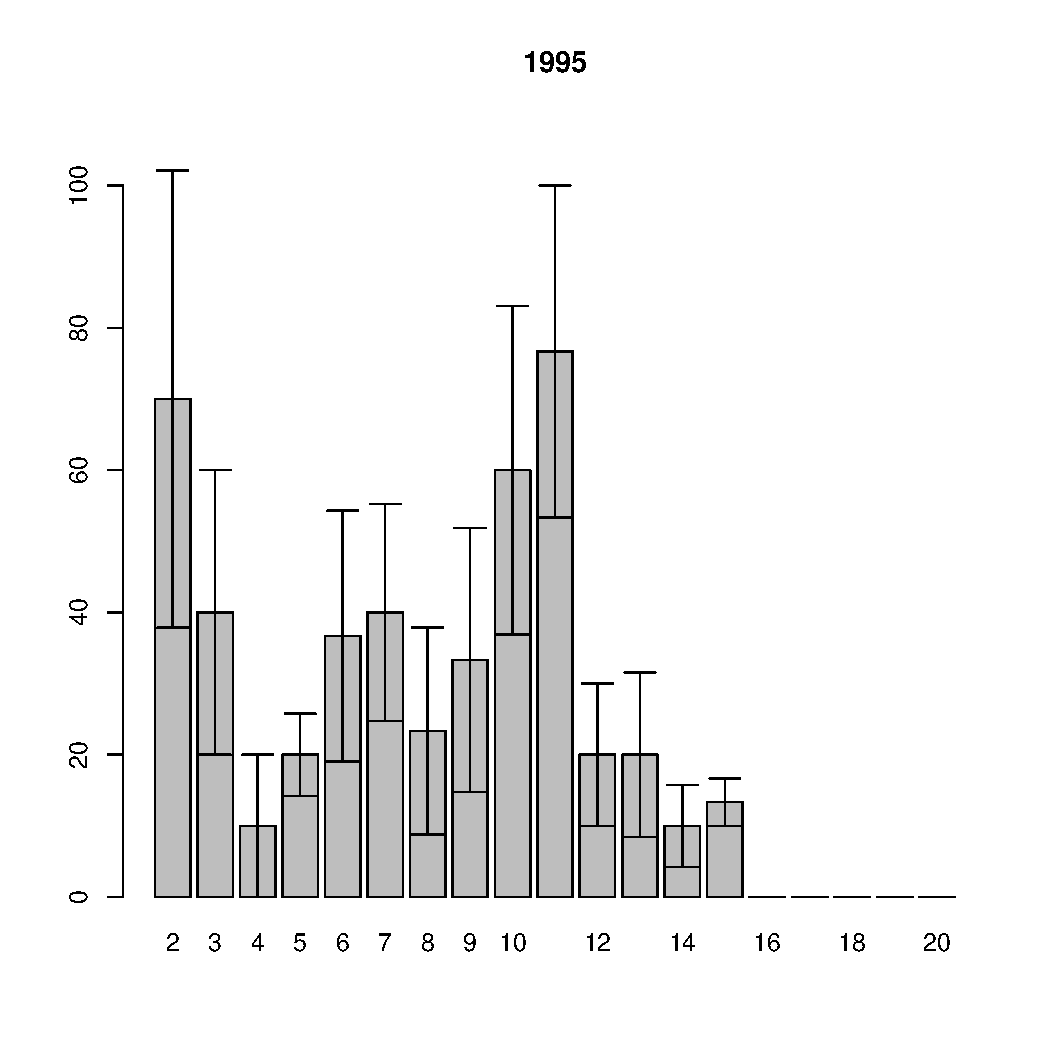
\includegraphics[width=65mm]{../White_Sea/Estuatiy_Luvenga/sizestr2_1995_.pdf}

\hfill
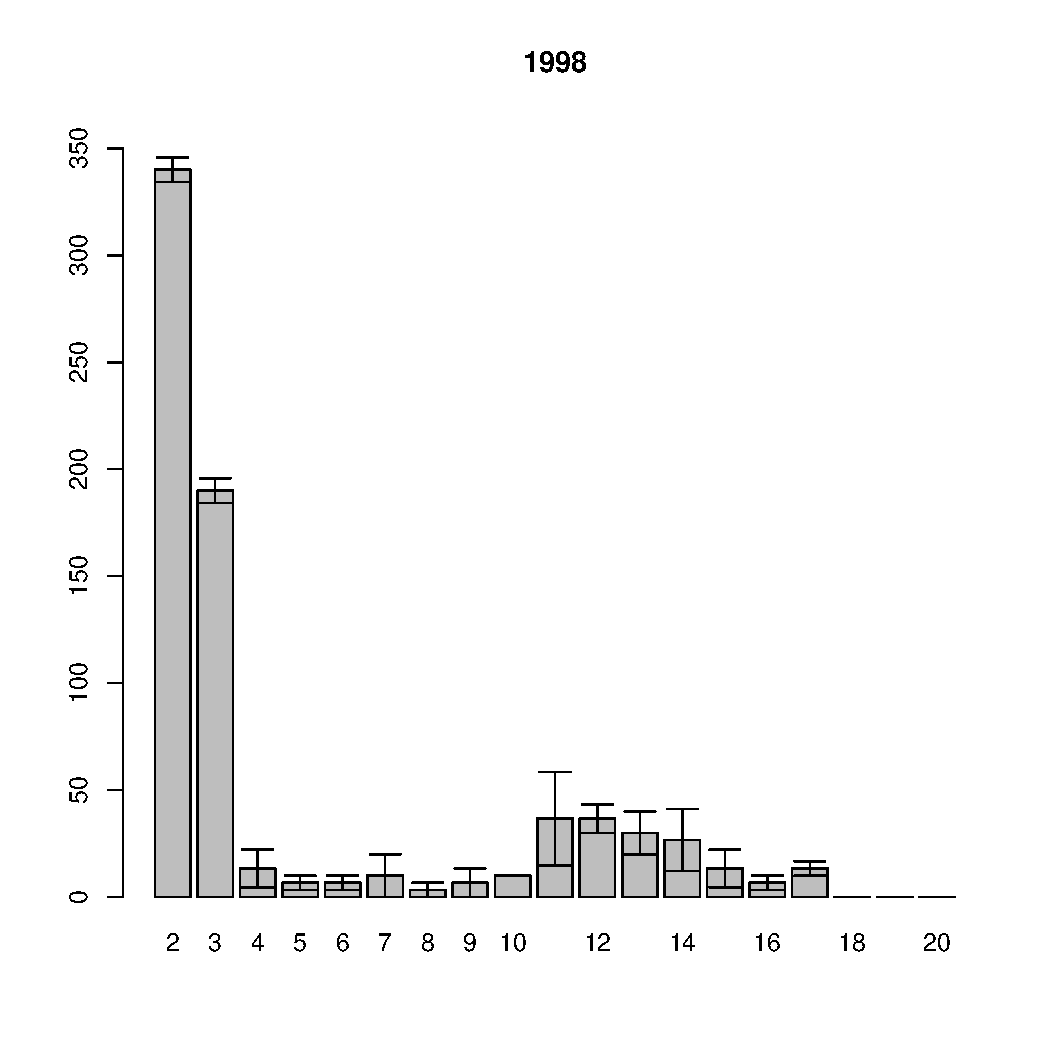
\includegraphics[width=65mm]{../White_Sea/Estuatiy_Luvenga/sizestr2_1998_.pdf}

\end{multicols}

%\smallskip


\begin{multicols}{3}
\hfill
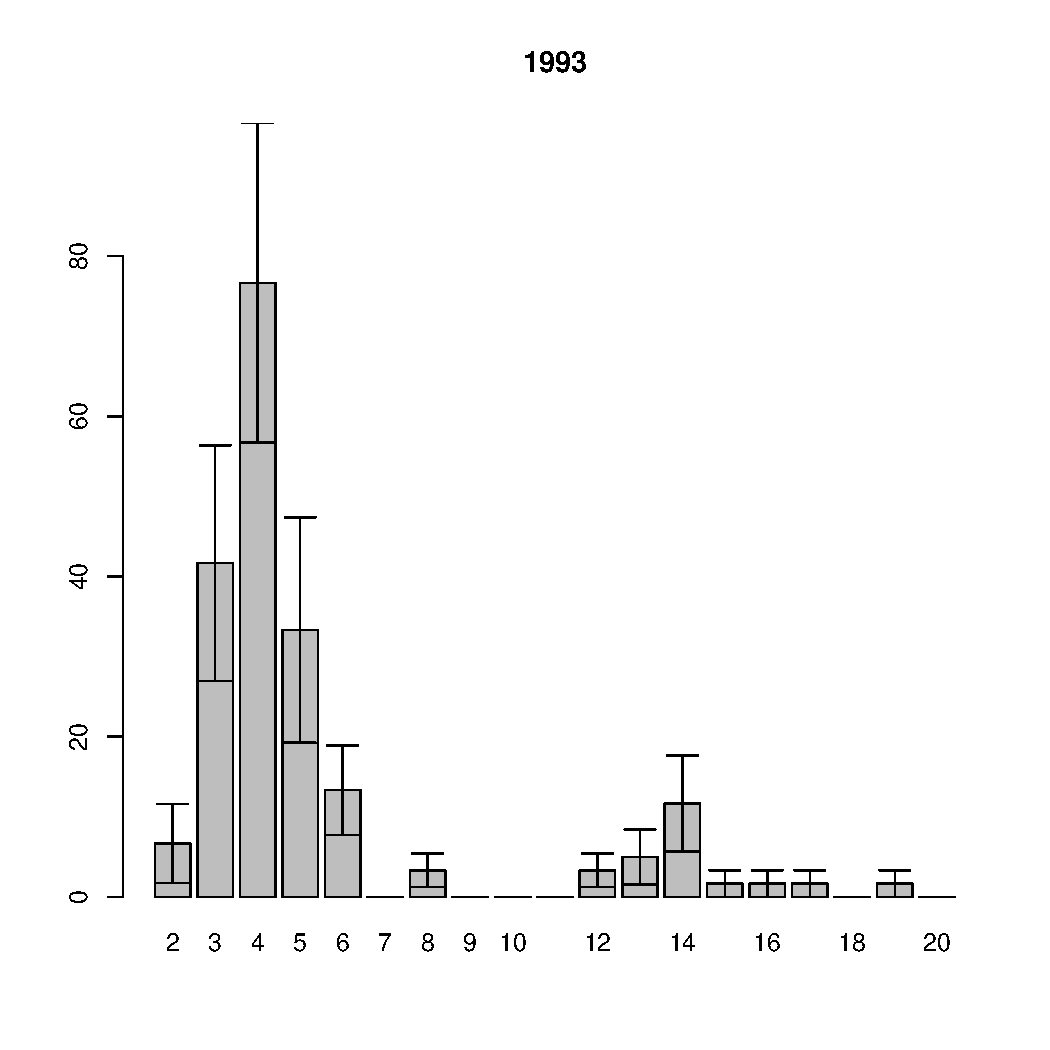
\includegraphics[width=65mm]{../White_Sea/Estuatiy_Luvenga/sizestr2_1993_.pdf}
\hfill
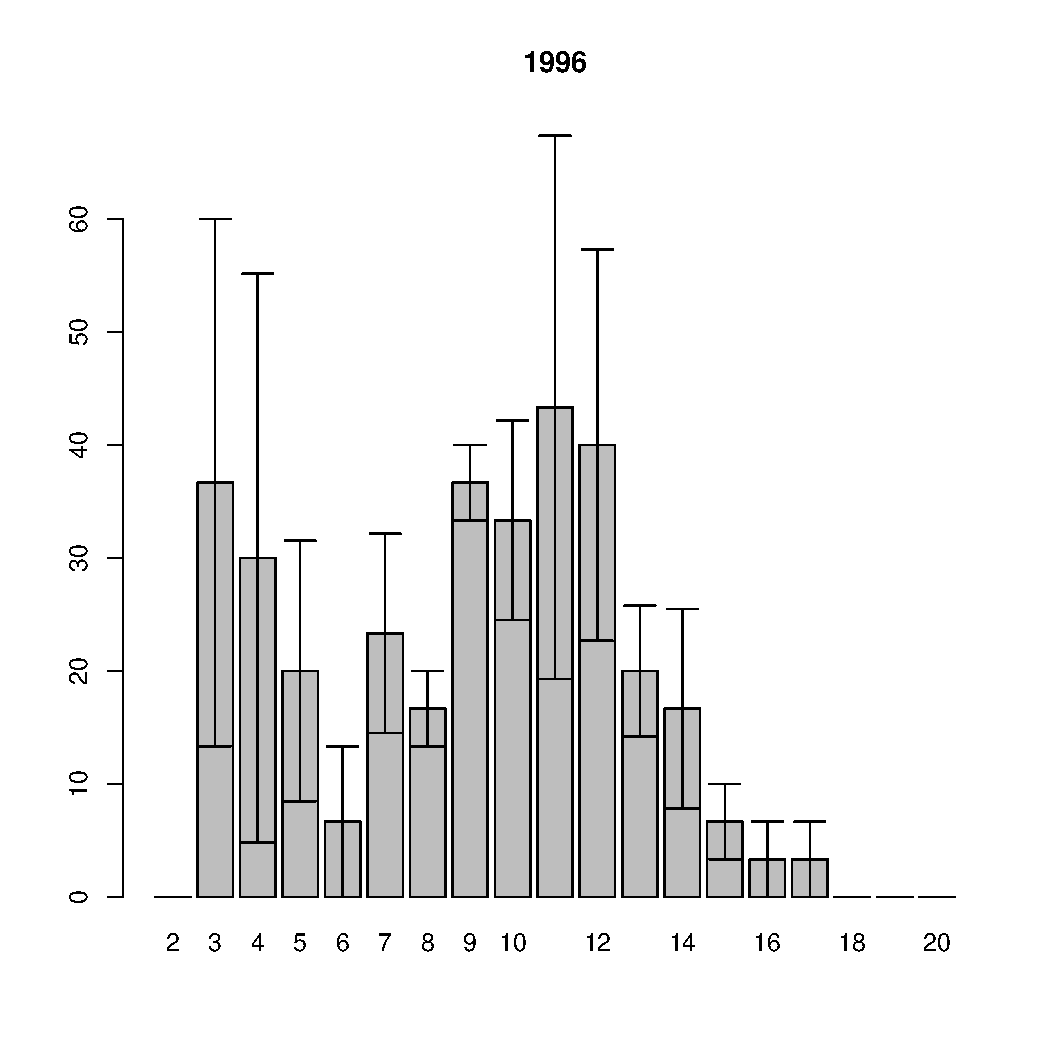
\includegraphics[width=65mm]{../White_Sea/Estuatiy_Luvenga/sizestr2_1996_.pdf}
\hfill
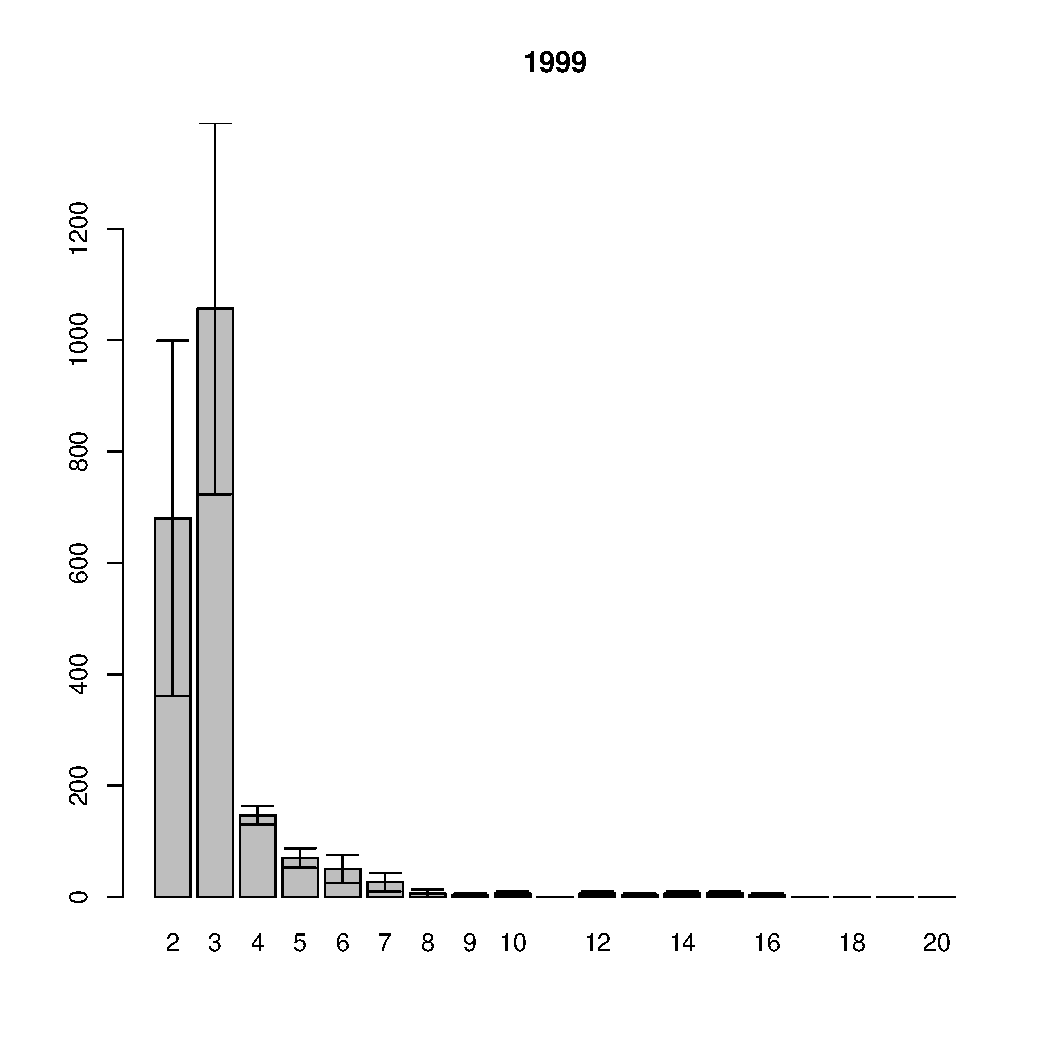
\includegraphics[width=65mm]{../White_Sea/Estuatiy_Luvenga/sizestr2_1999_.pdf}

\end{multicols}

%\smallskip

\begin{multicols}{3}
\hfill
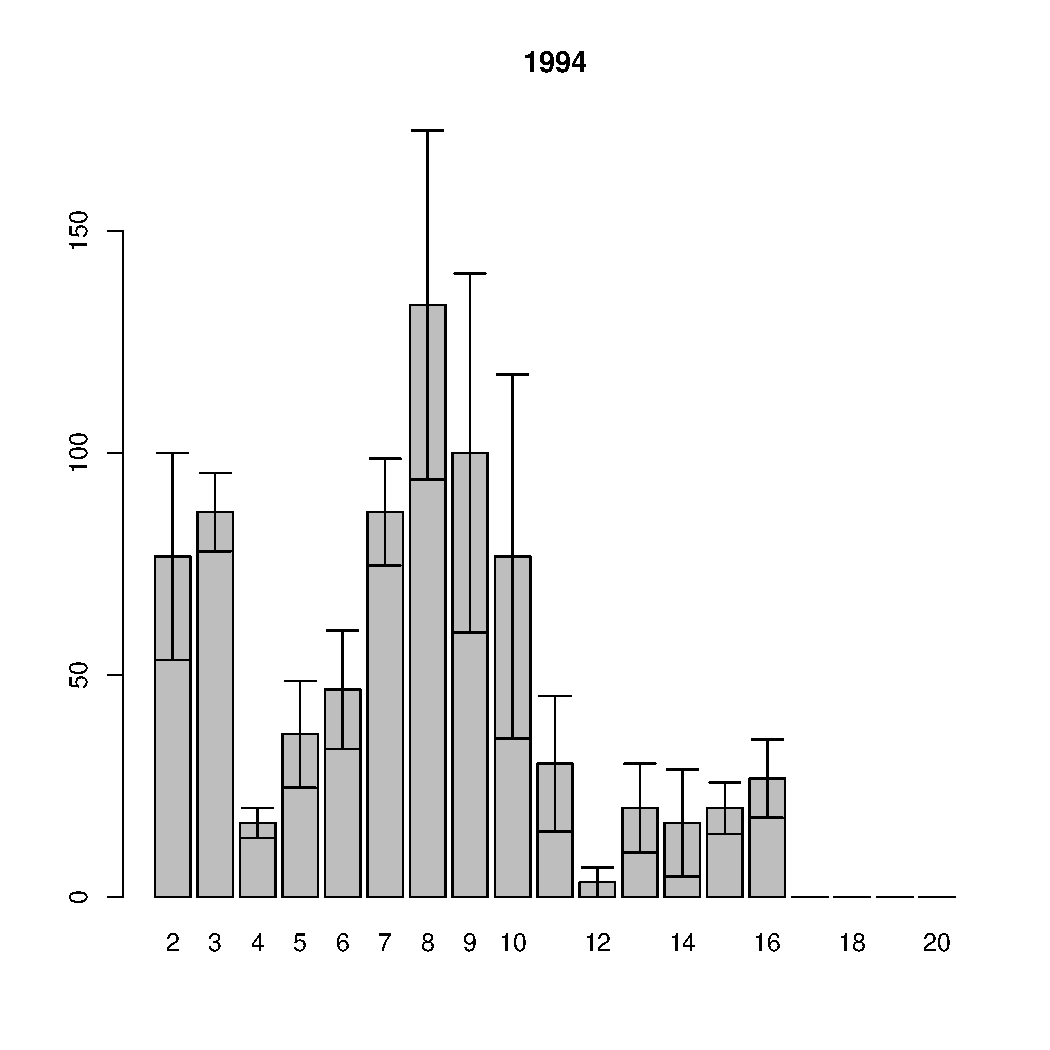
\includegraphics[width=65mm]{../White_Sea/Estuatiy_Luvenga/sizestr2_1994_.pdf}
\hfill
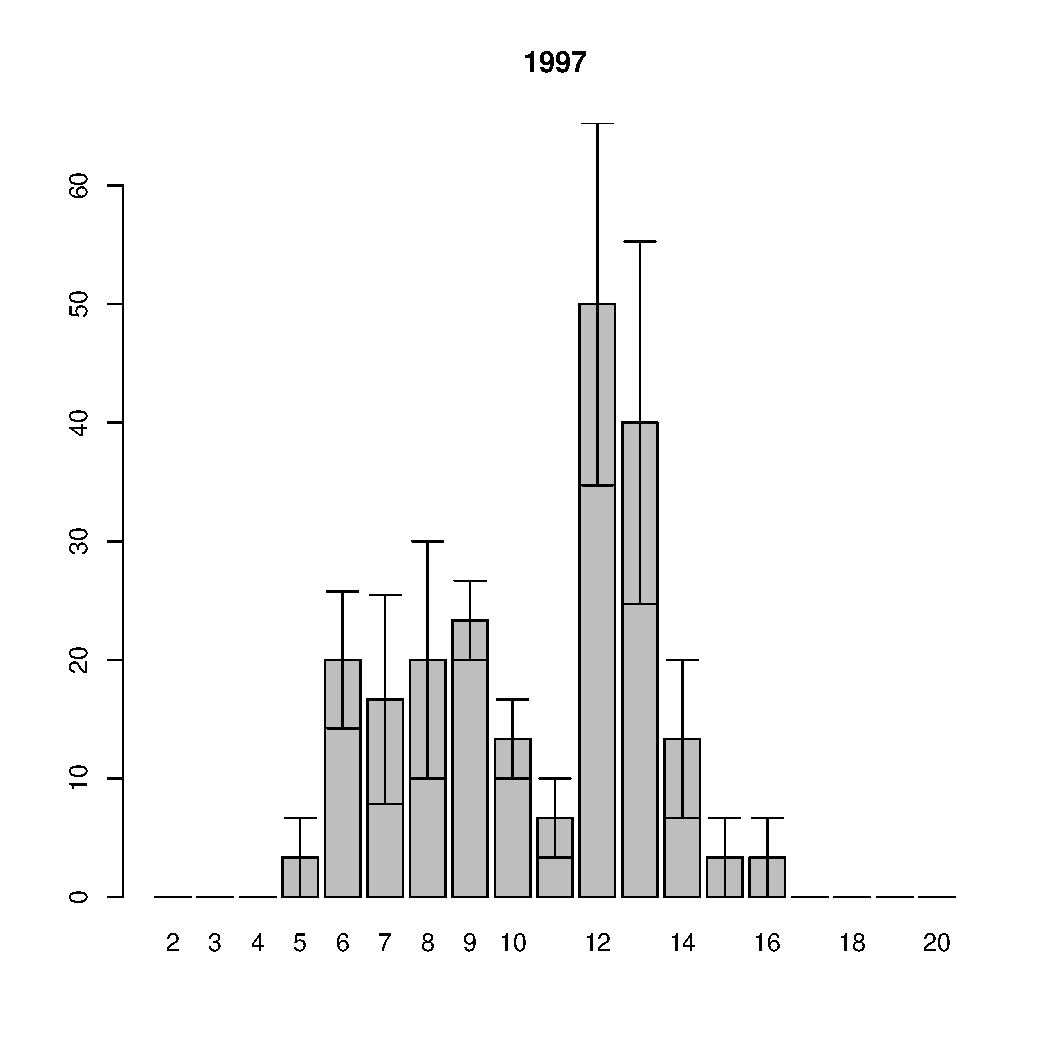
\includegraphics[width=65mm]{../White_Sea/Estuatiy_Luvenga/sizestr2_1997_.pdf}
\hfill
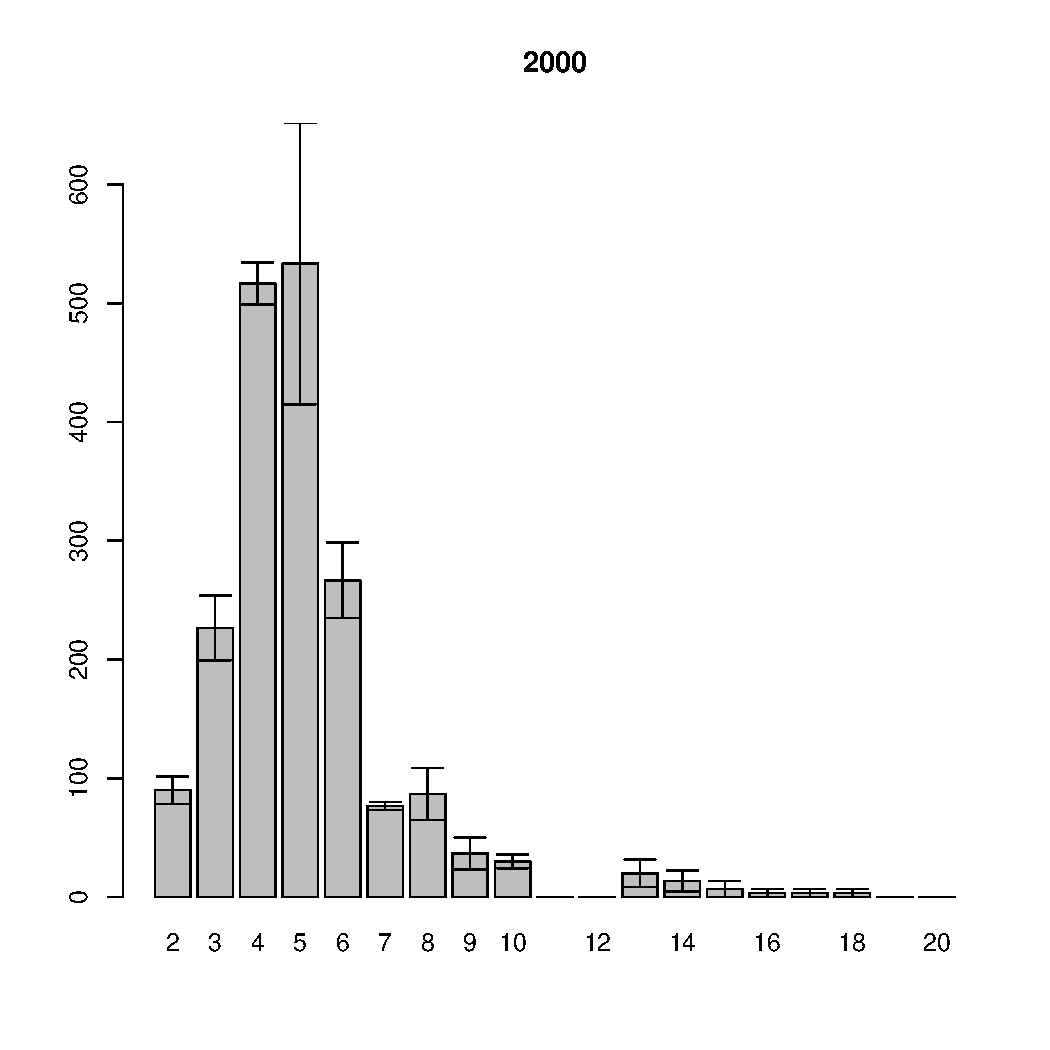
\includegraphics[width=65mm]{../White_Sea/Estuatiy_Luvenga/sizestr2_2000_.pdf}
\end{multicols}

%\smallskip


\caption{Размерная структура {\it Macoma balthica} в СГЛ эстуария р. Лувеньги}
\label{ris:size_str_estuary_Luv}
\end{figure}


\begin{figure}[h]

\begin{multicols}{3}
\hfill
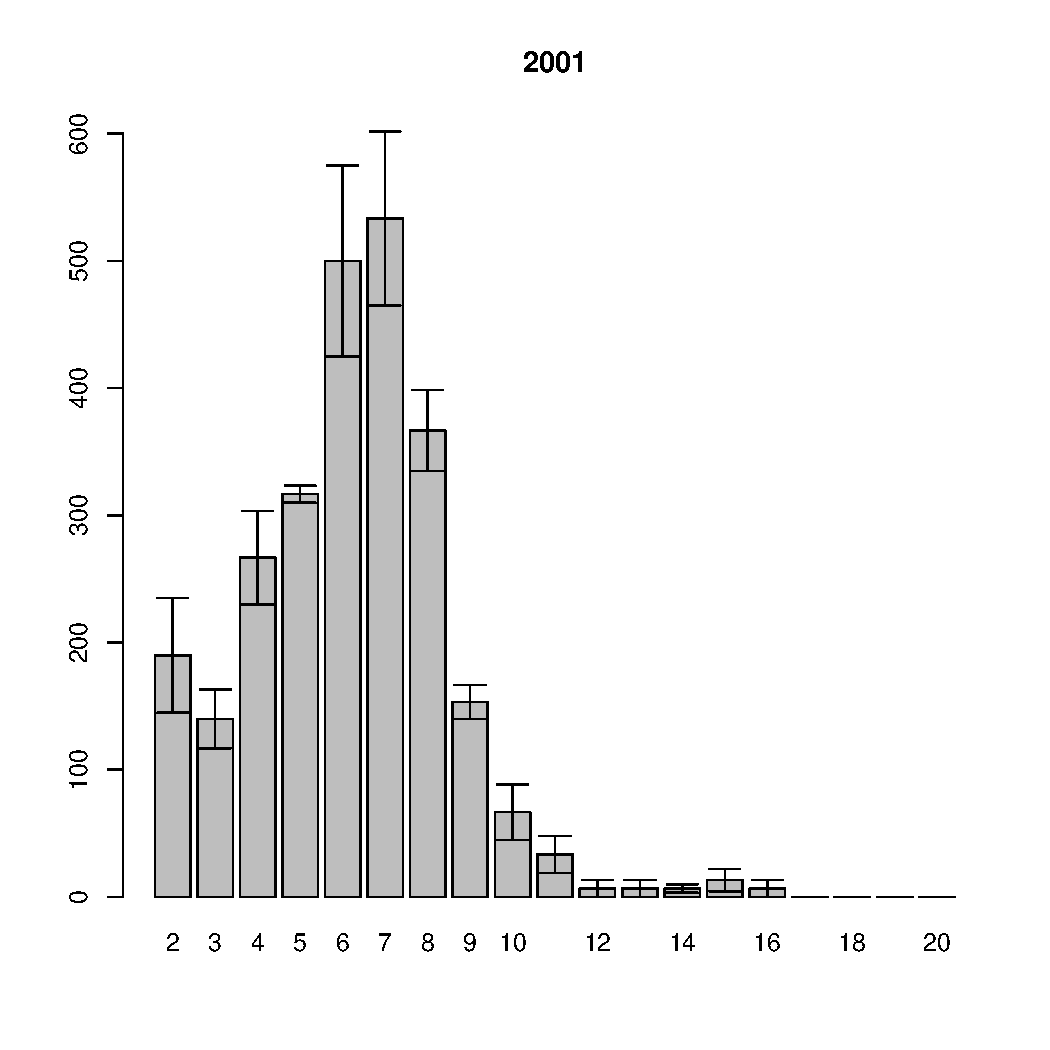
\includegraphics[width=65mm]{../White_Sea/Estuatiy_Luvenga/sizestr2_2001_.pdf}
\hfill
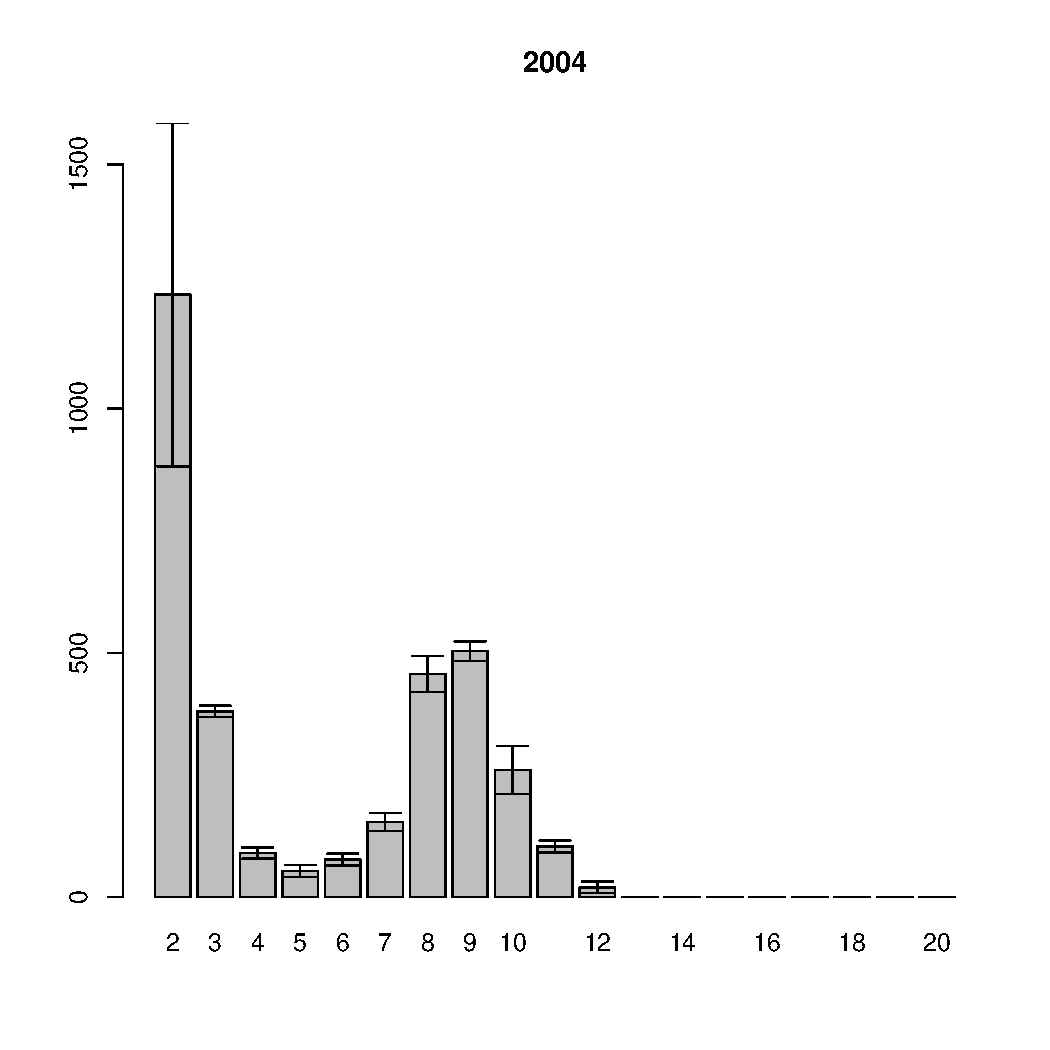
\includegraphics[width=65mm]{../White_Sea/Estuatiy_Luvenga/sizestr2_2004_.pdf}
\hfill
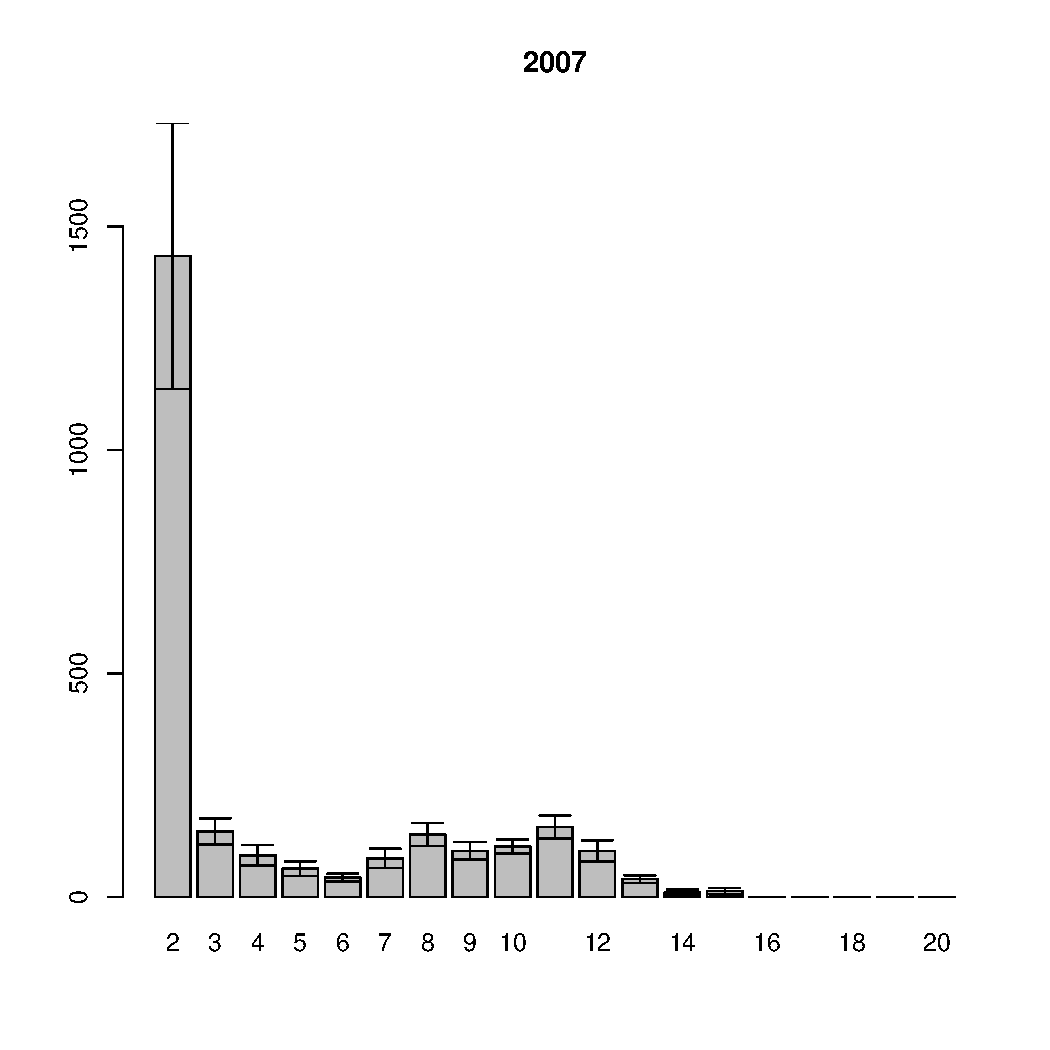
\includegraphics[width=65mm]{../White_Sea/Estuatiy_Luvenga/sizestr2_2007_.pdf}
\end{multicols}

\begin{multicols}{3}
\hfill
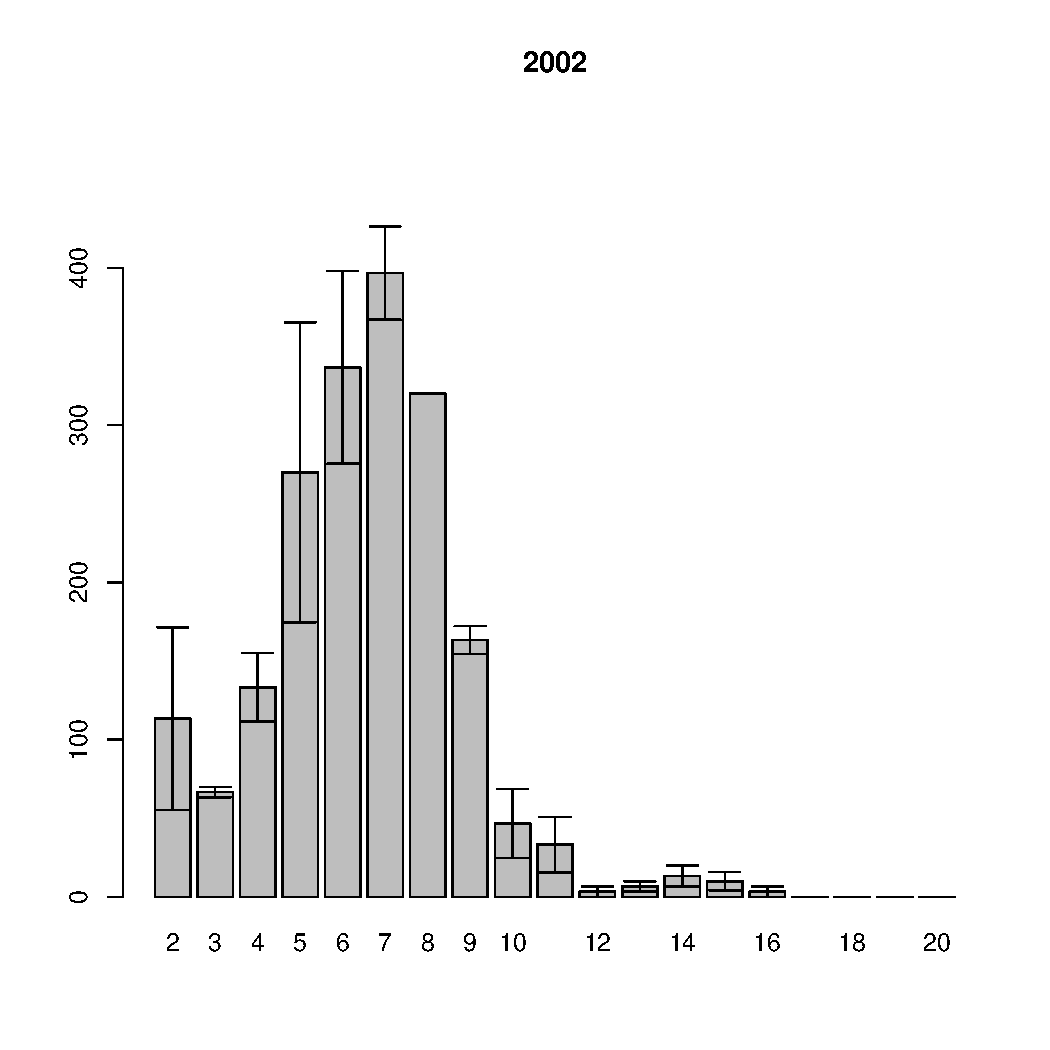
\includegraphics[width=65mm]{../White_Sea/Estuatiy_Luvenga/sizestr2_2002_.pdf}
\hfill
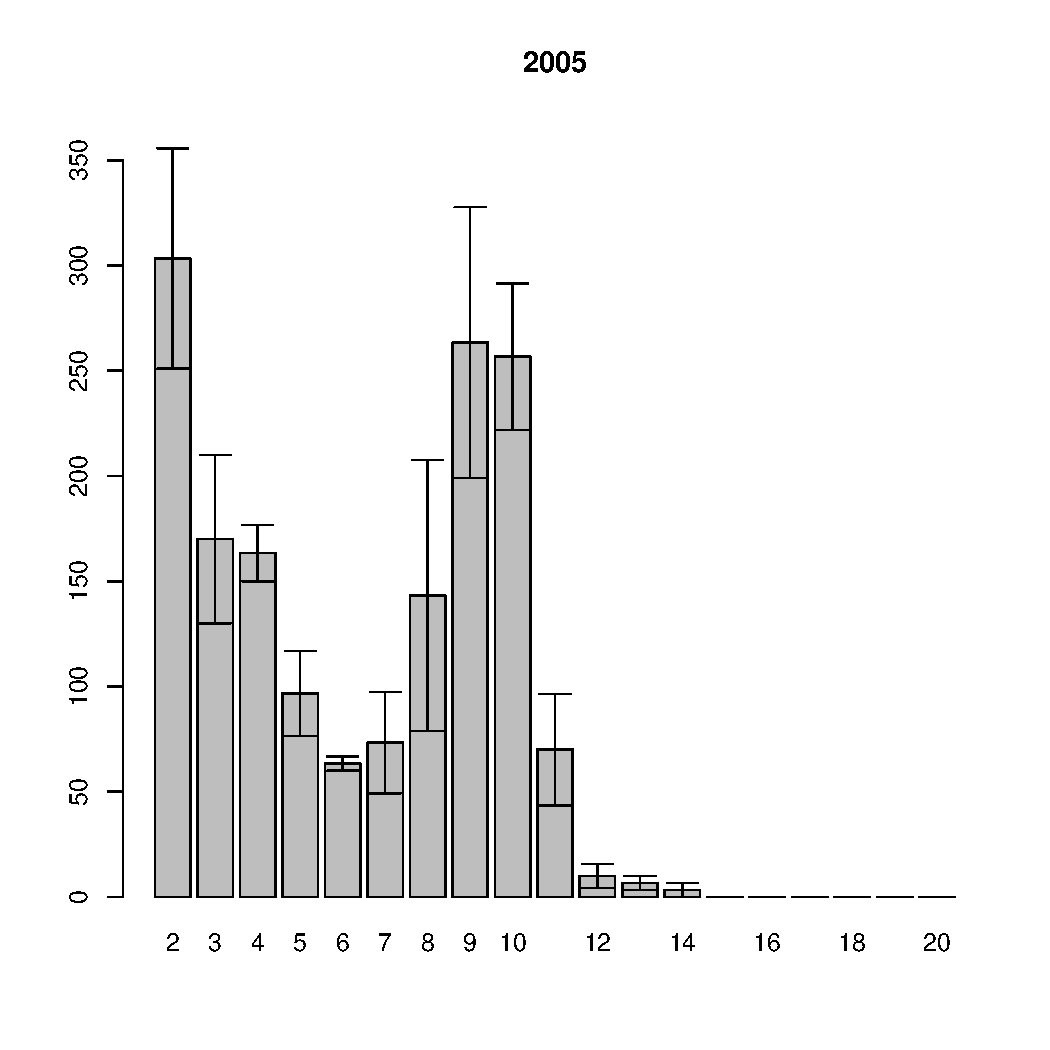
\includegraphics[width=65mm]{../White_Sea/Estuatiy_Luvenga/sizestr2_2005_.pdf}
\hfill
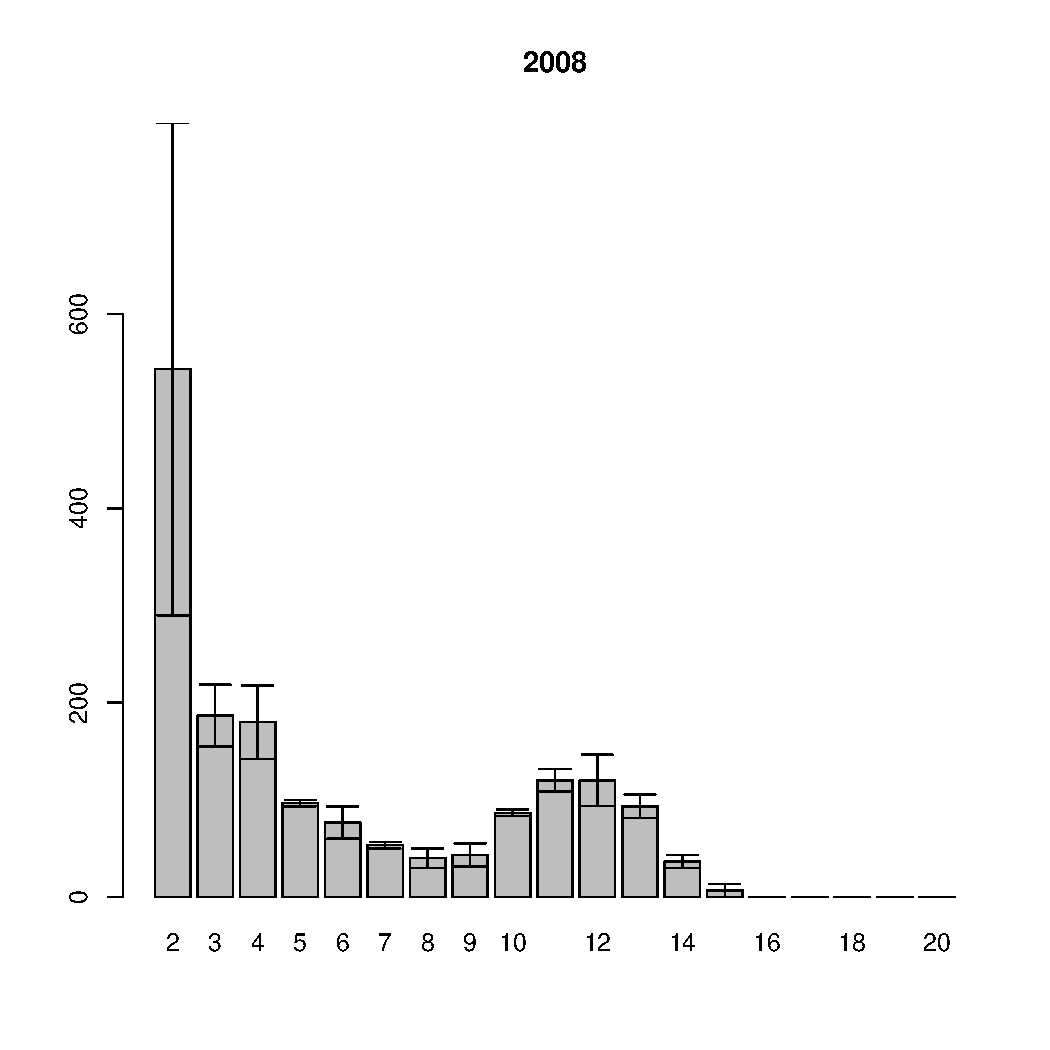
\includegraphics[width=65mm]{../White_Sea/Estuatiy_Luvenga/sizestr2_2008_.pdf}
\end{multicols}

%\smallskip


\begin{multicols}{3}
\hfill
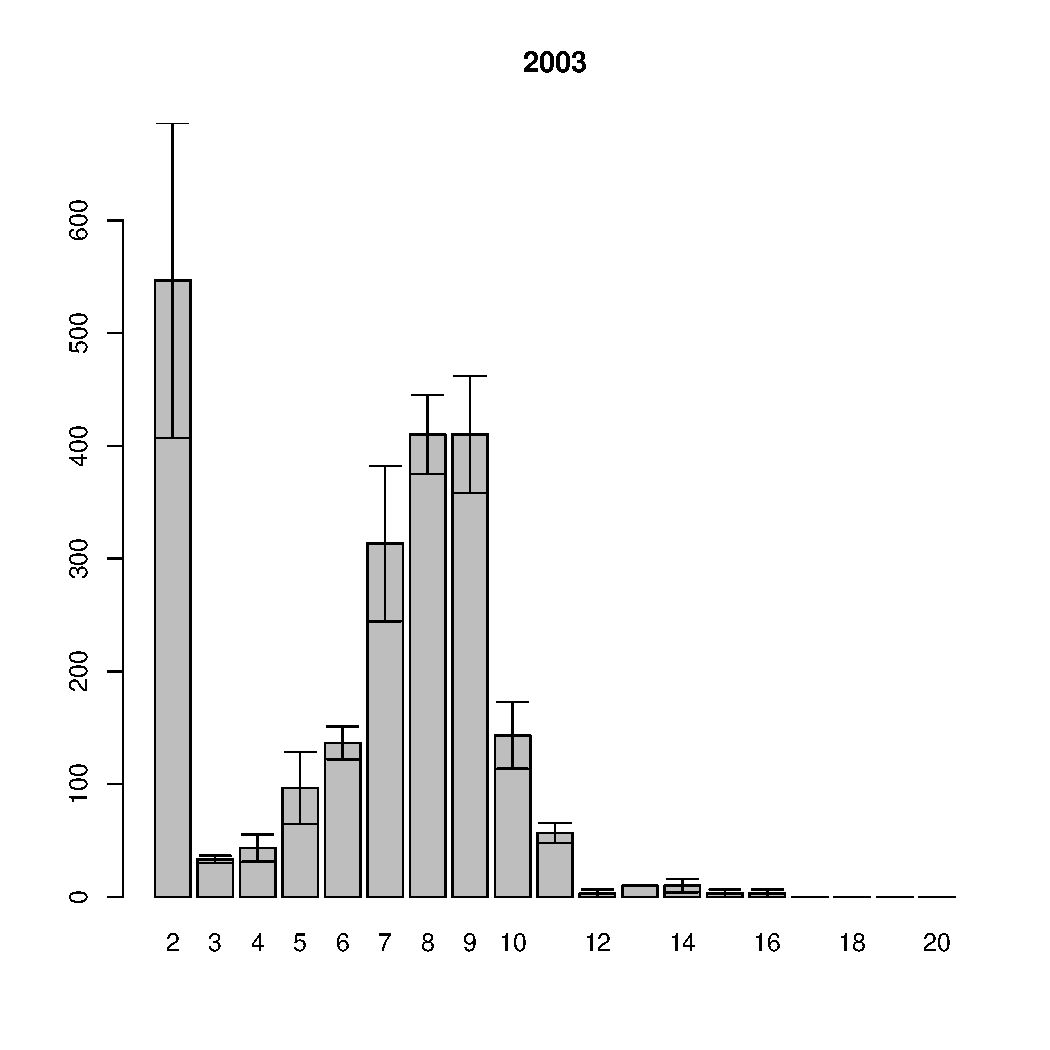
\includegraphics[width=65mm]{../White_Sea/Estuatiy_Luvenga/sizestr2_2003_.pdf}
\hfill
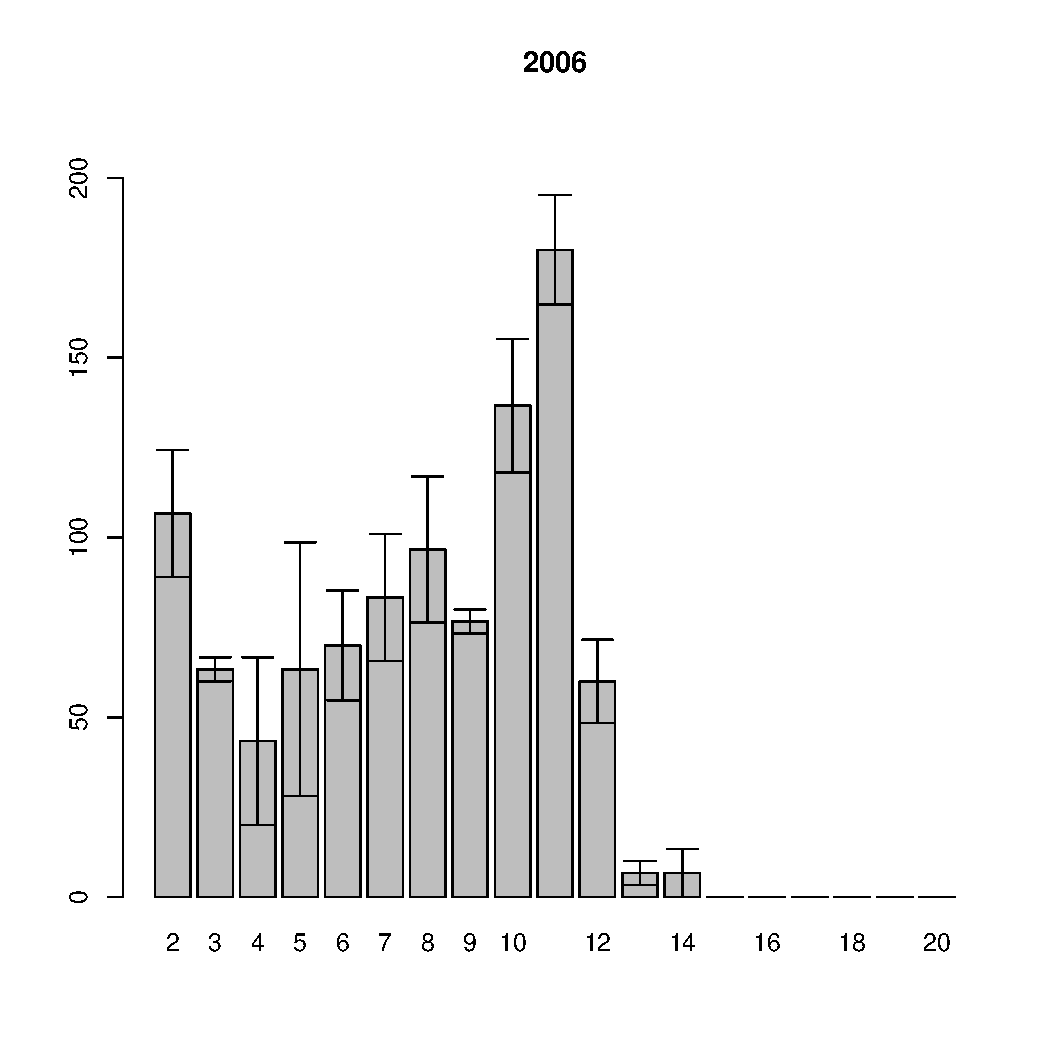
\includegraphics[width=65mm]{../White_Sea/Estuatiy_Luvenga/sizestr2_2006_.pdf}
\hfill
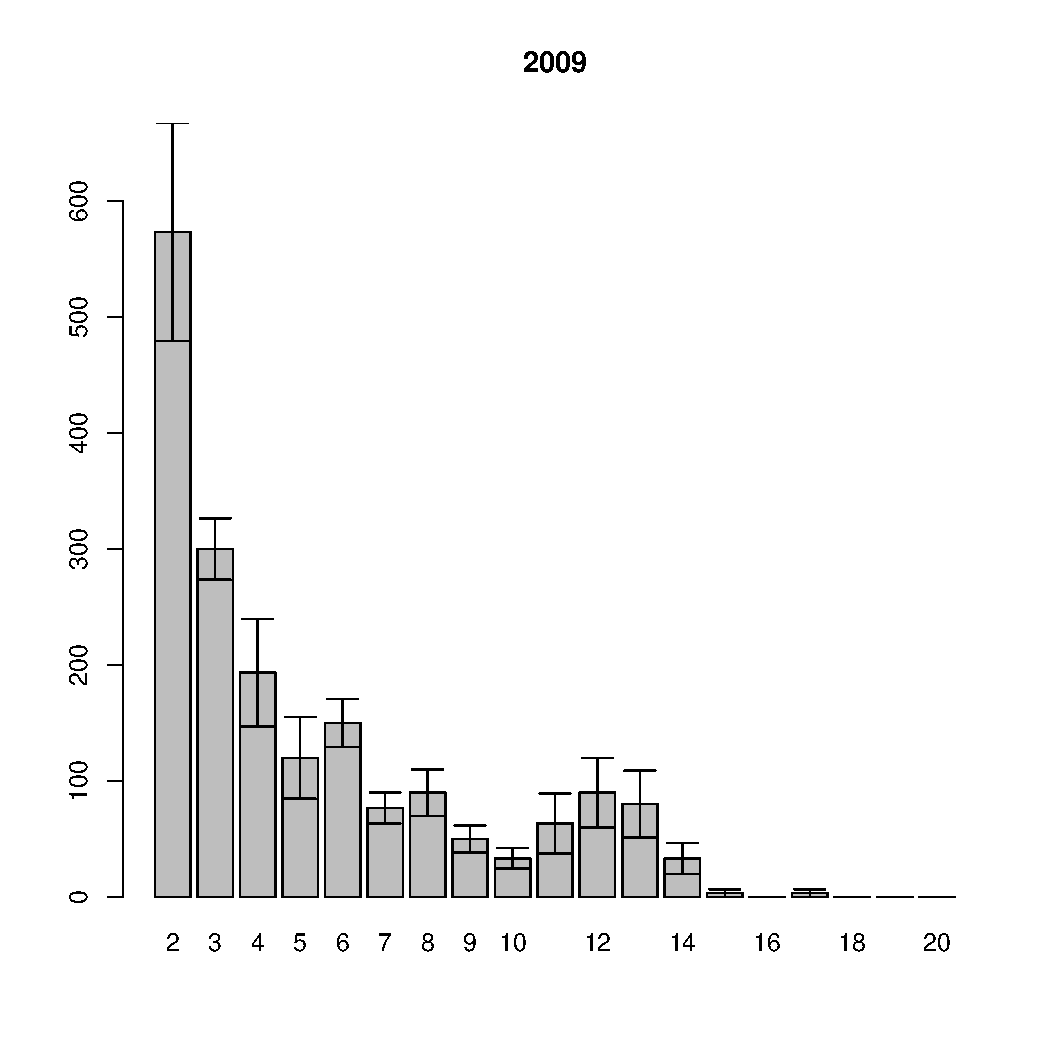
\includegraphics[width=65mm]{../White_Sea/Estuatiy_Luvenga/sizestr2_2009_.pdf}
\end{multicols}

%\smallskip


%\caption{Размерная структура {\it Macoma balthica} в СГЛ эстуария р. Лувеньги}
%\label{ris:size_str_estuaty_Luv}
\begin{center}
Рис. \ref{ris:size_str_estuary_Luv} (продолжение). Размерная структура {\it Macoma balthica} в СГЛ эстуария р. Лувеньги

\end{center}
\end{figure}


\begin{figure}[h]

\begin{multicols}{3}
\hfill
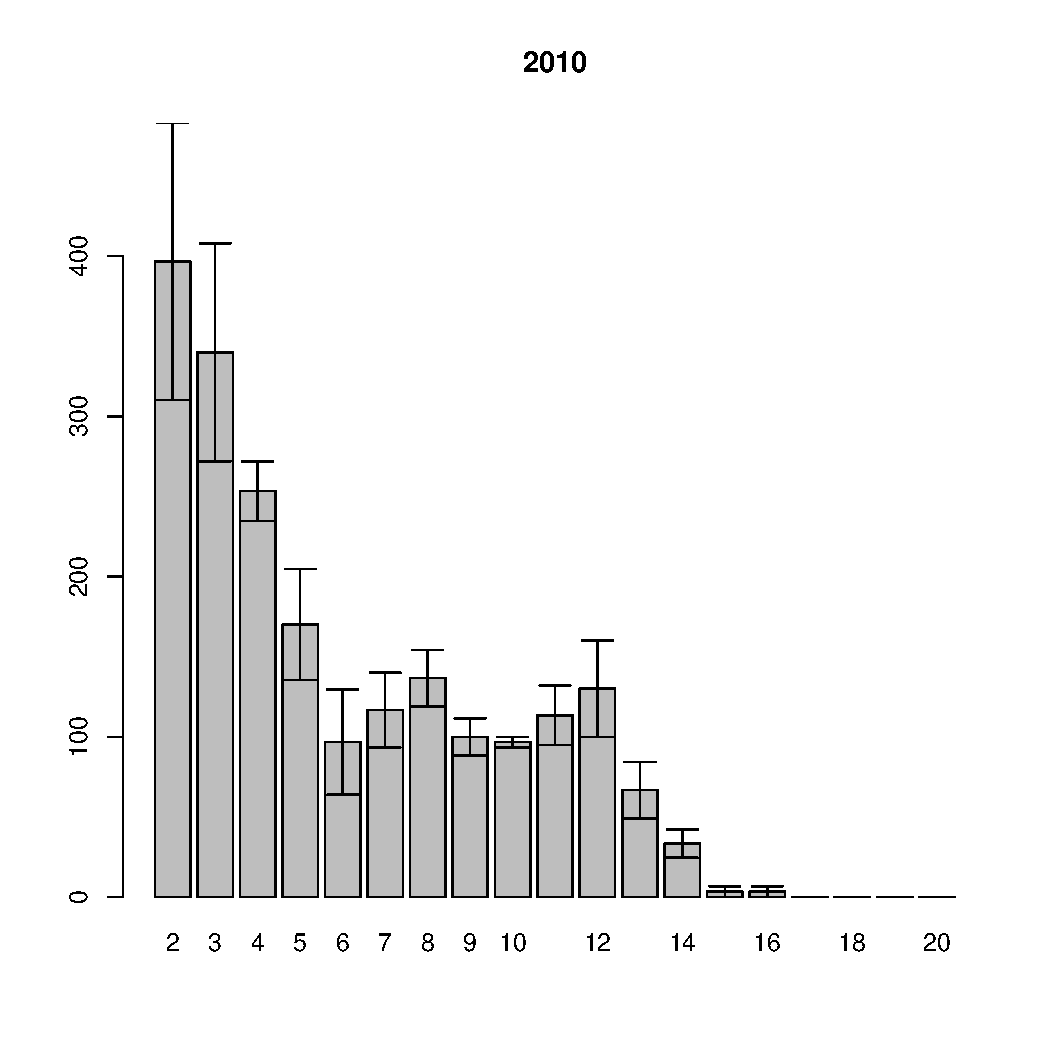
\includegraphics[width=65mm]{../White_Sea/Estuatiy_Luvenga/sizestr2_2010_.pdf}
\hfill
%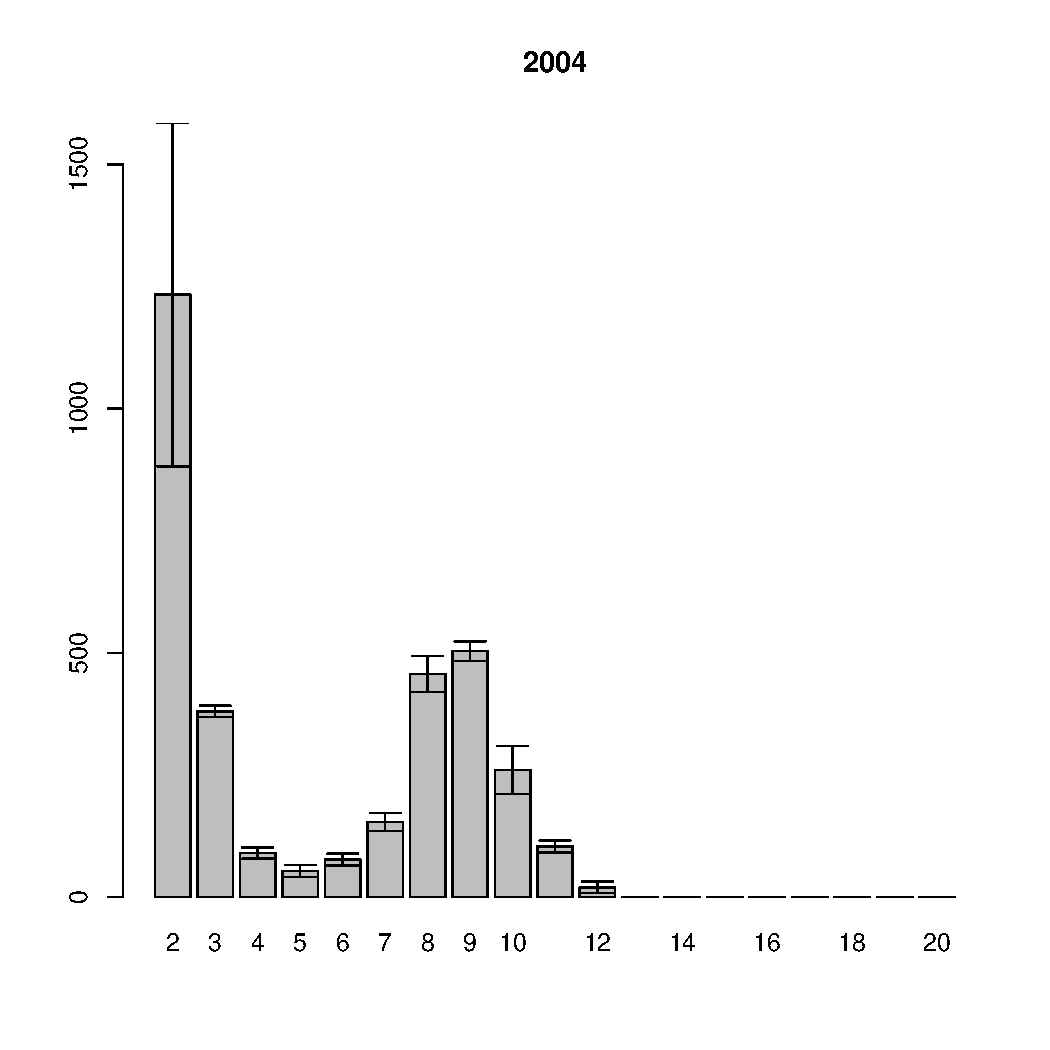
\includegraphics[width=65mm]{../White_Sea/Estuatiy_Luvenga/sizestr2_2004_.pdf}
%\hfill
%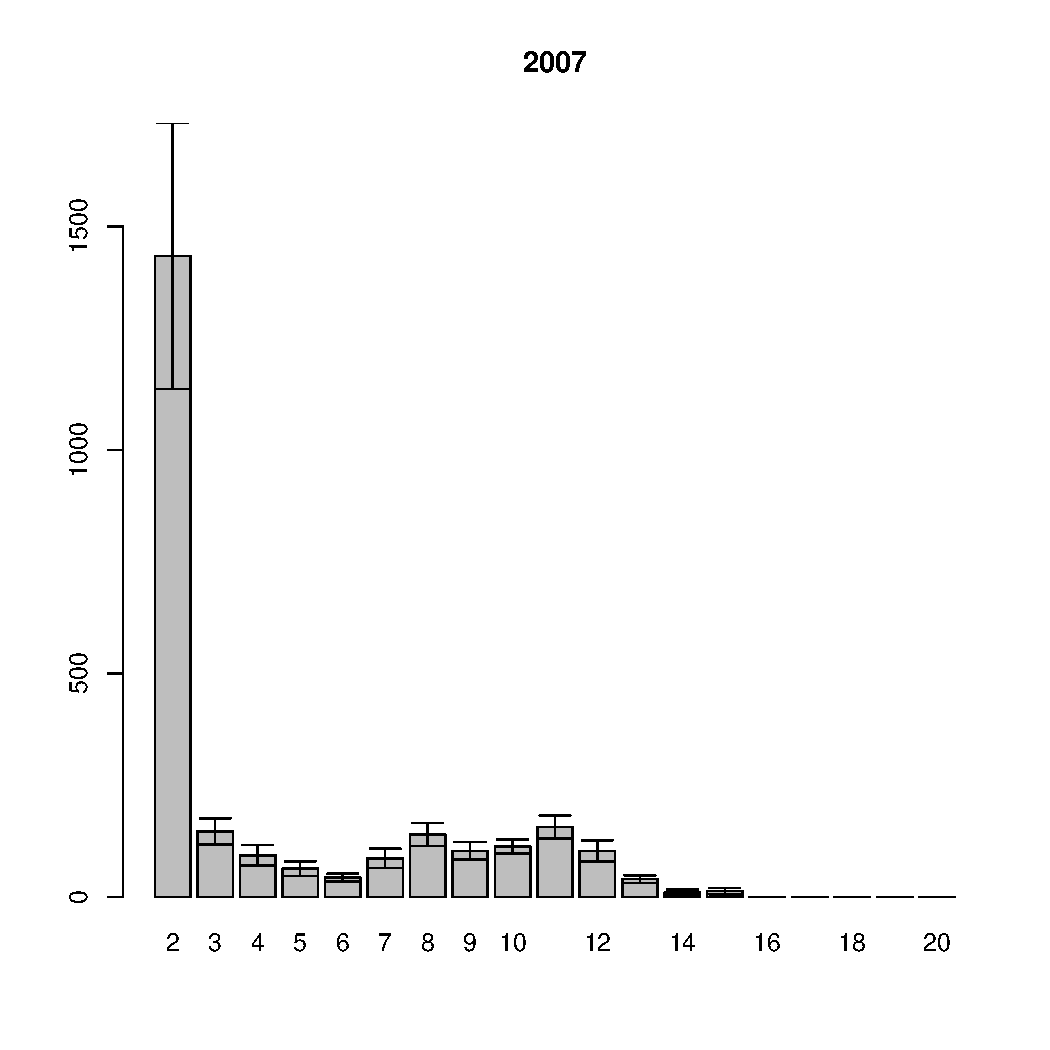
\includegraphics[width=65mm]{../White_Sea/Estuatiy_Luvenga/sizestr2_2007_.pdf}
\end{multicols}

\begin{multicols}{3}
\hfill
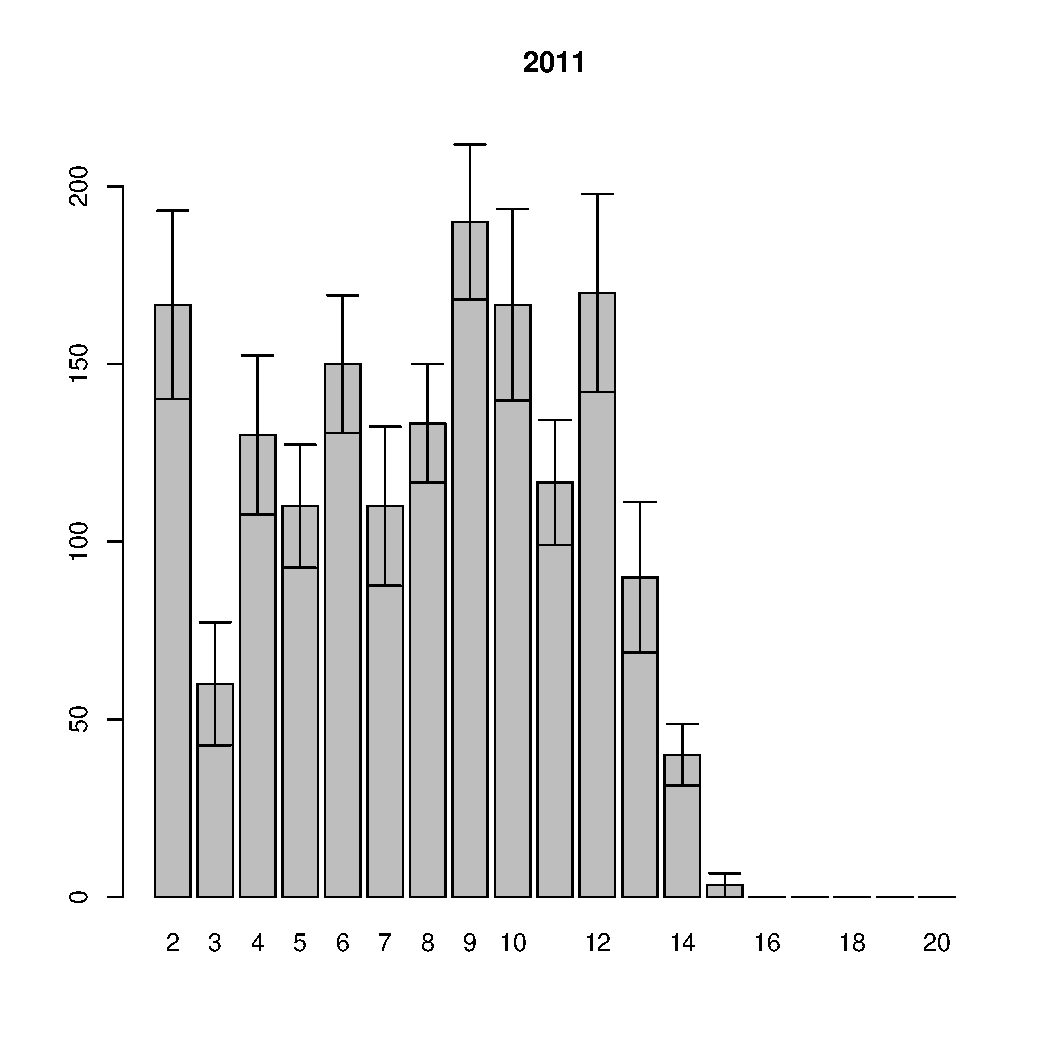
\includegraphics[width=65mm]{../White_Sea/Estuatiy_Luvenga/sizestr2_2011_.pdf}
%\hfill
%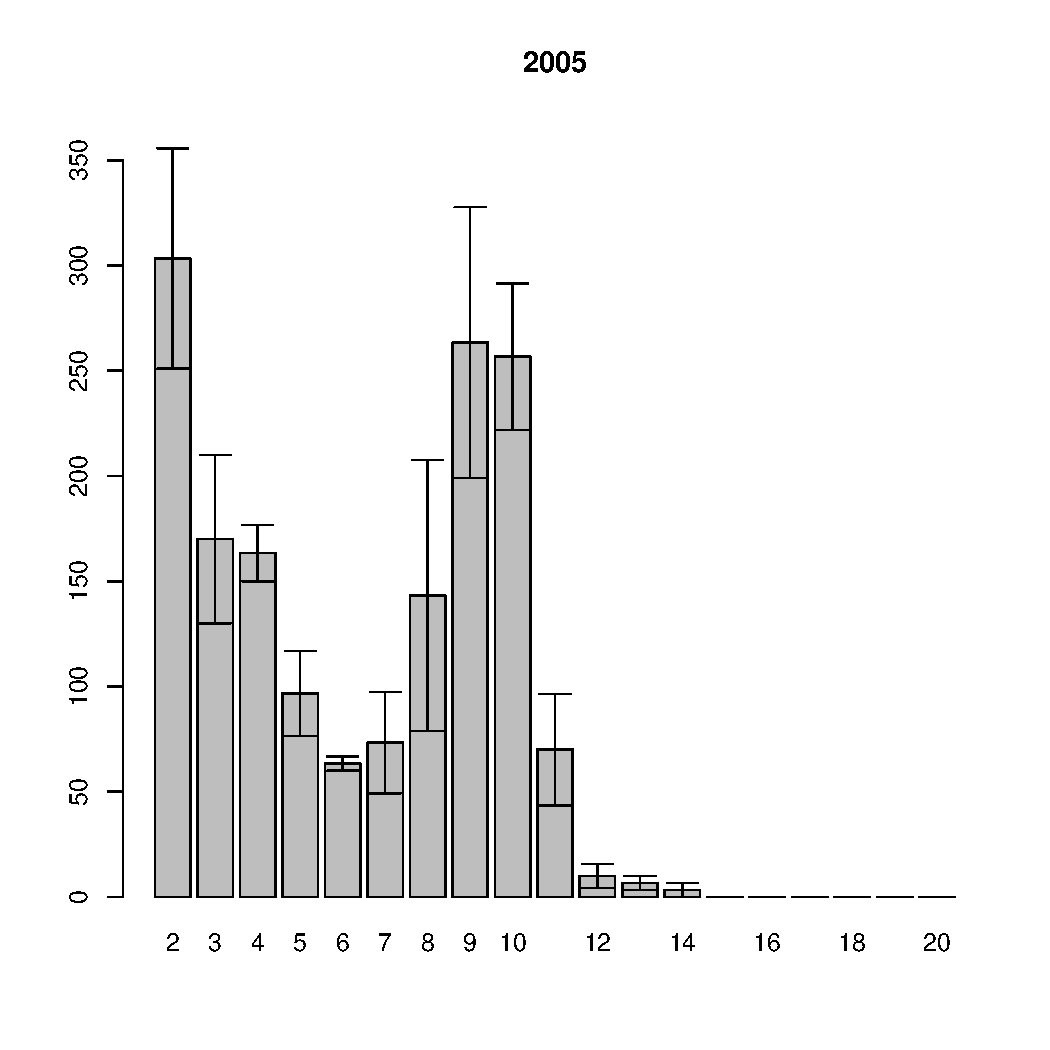
\includegraphics[width=65mm]{../White_Sea/Estuatiy_Luvenga/sizestr2_2005_.pdf}
%\hfill
%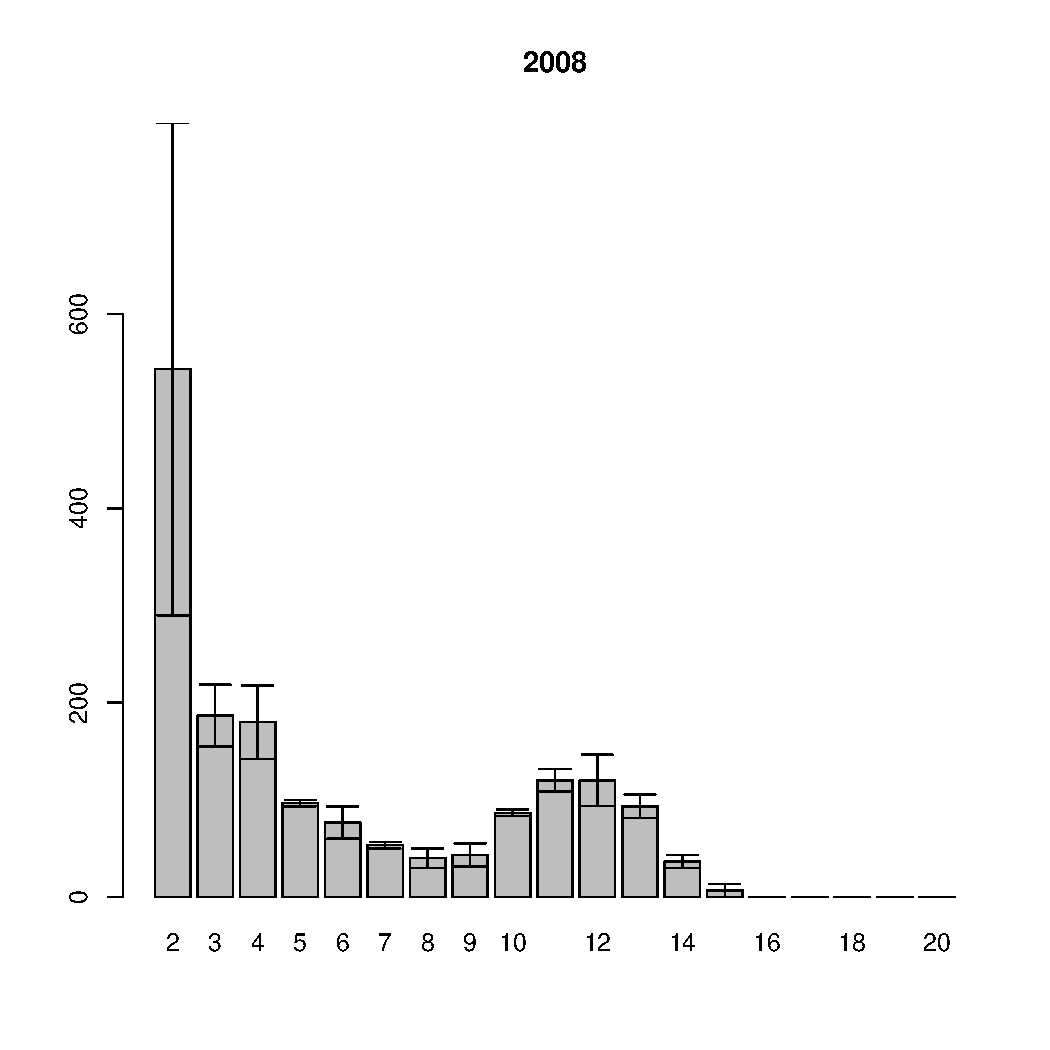
\includegraphics[width=65mm]{../White_Sea/Estuatiy_Luvenga/sizestr2_2008_.pdf}
\end{multicols}

%\smallskip


\begin{multicols}{3}
\hfill
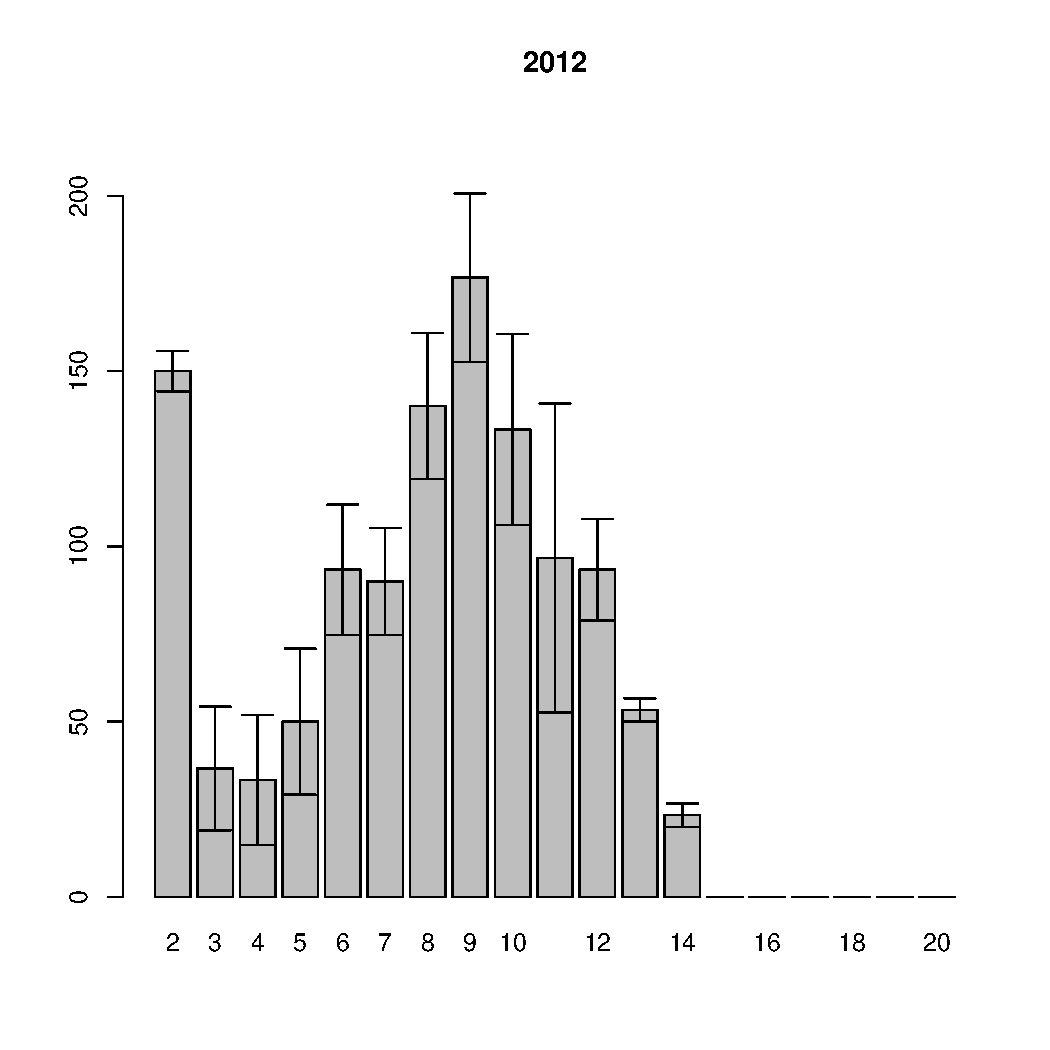
\includegraphics[width=65mm]{../White_Sea/Estuatiy_Luvenga/sizestr2_2012_.pdf}
%\hfill
%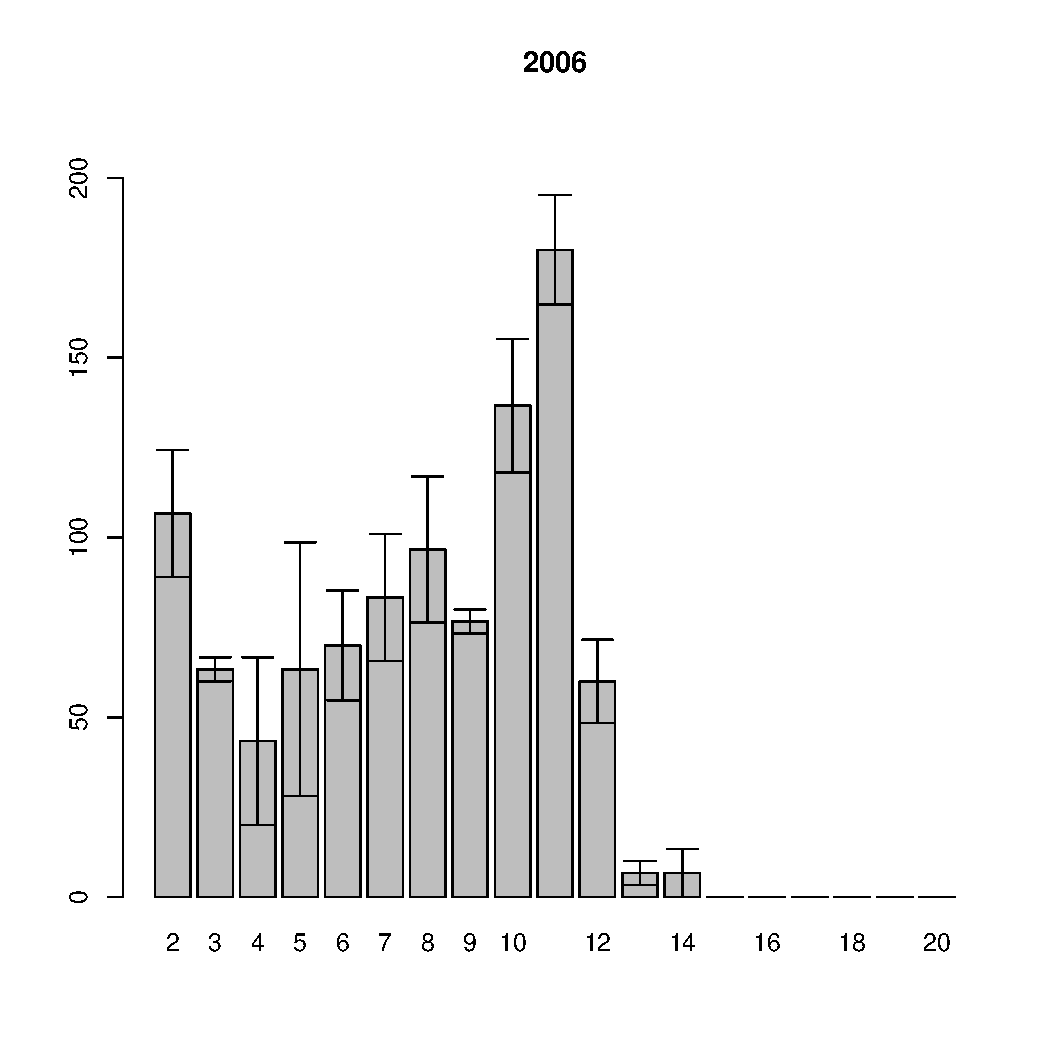
\includegraphics[width=65mm]{../White_Sea/Estuatiy_Luvenga/sizestr2_2006_.pdf}
%\hfill
%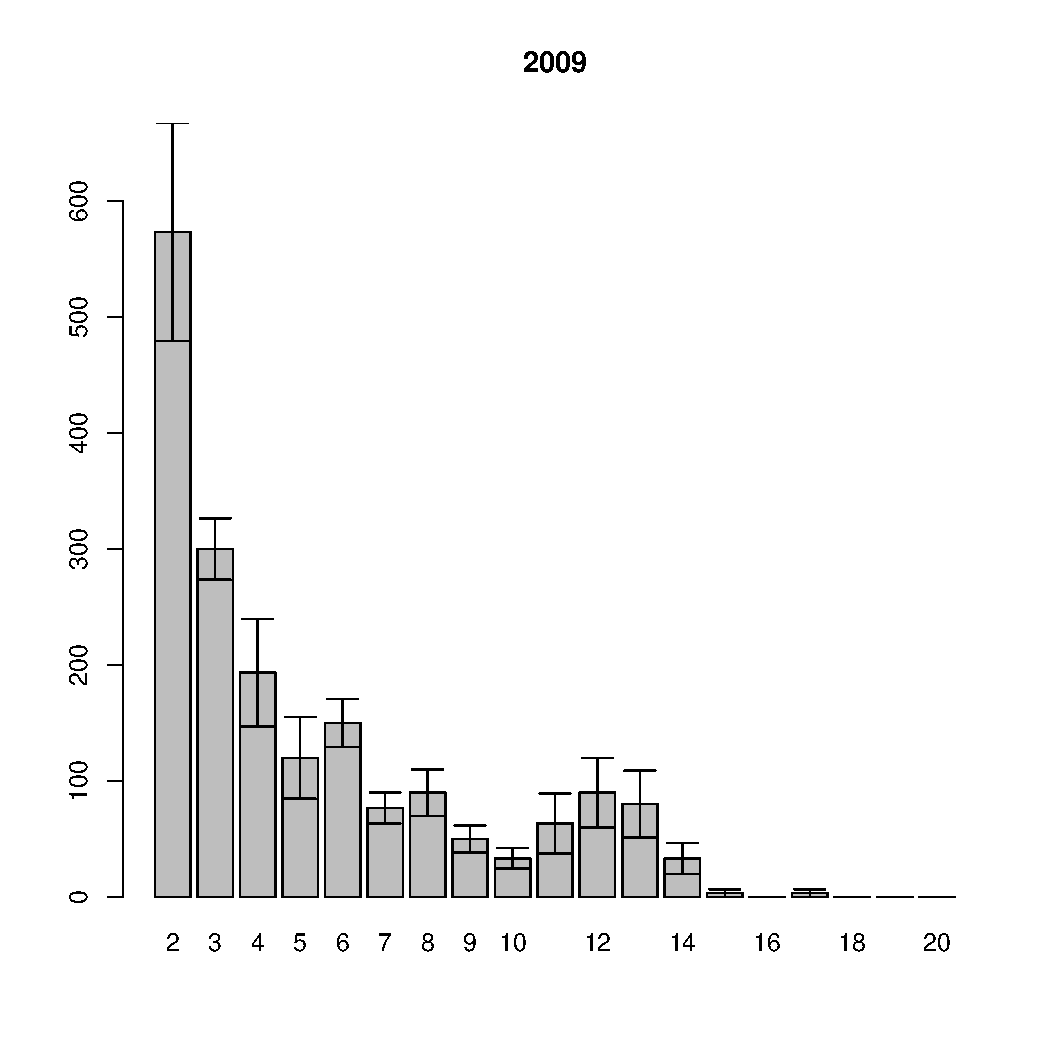
\includegraphics[width=65mm]{../White_Sea/Estuatiy_Luvenga/sizestr2_2009_.pdf}
\end{multicols}

%\smallskip


%\caption{Размерная структура {\it Macoma balthica} в СГЛ эстуария р. Лувеньги}
%\label{ris:size_str_estuaty_Luv}
\begin{center}
Рис. \ref{ris:size_str_estuary_Luv} (продолжение). Размерная структура {\it Macoma balthica} в СГЛ эстуария р. Лувеньги

\end{center}
\end{figure}





		\subsection{Максимальный размер особей в поселениях}


\newpage
\begin{figure}[h]

\begin{minipage}[b]{.46\linewidth}
%Фигурка в первом ряду слева размер отведенный под весь этот объект -- 0.46 от ширины строки
%Параметр [b] означает, что выравнивание этих министраниц будет по нижнему краю
\begin{center}
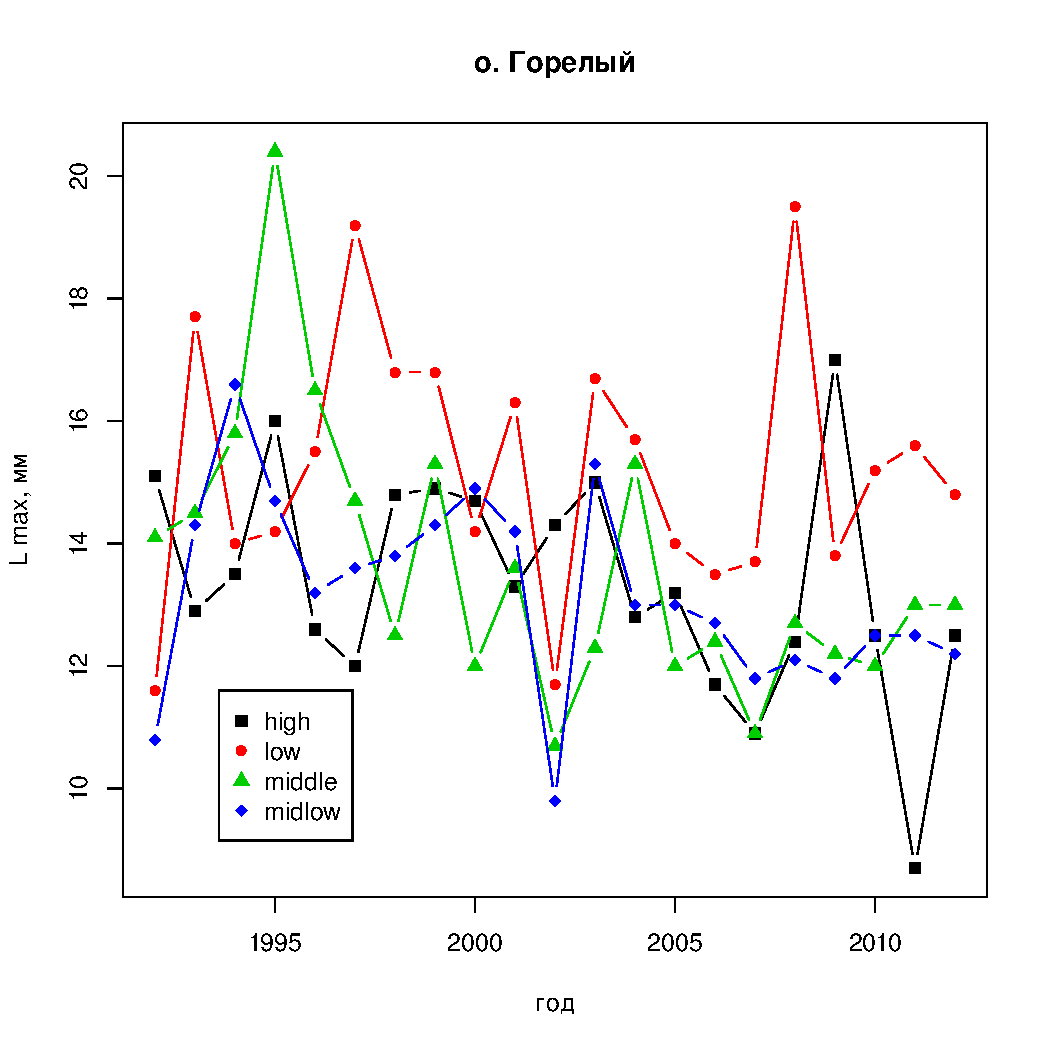
\includegraphics[width=65mm]{../White_Sea/Luvenga_Goreliy/L_max.pdf}
\end{center}
\end{minipage}
%
\hfil %Это пружинка отодвигающая рисунки друг от друга
%
\begin{minipage}[b]{.46\linewidth}
%Следующий рисунок - первый ряд справа %DUNGEON S_4 \ AB
\begin{center}
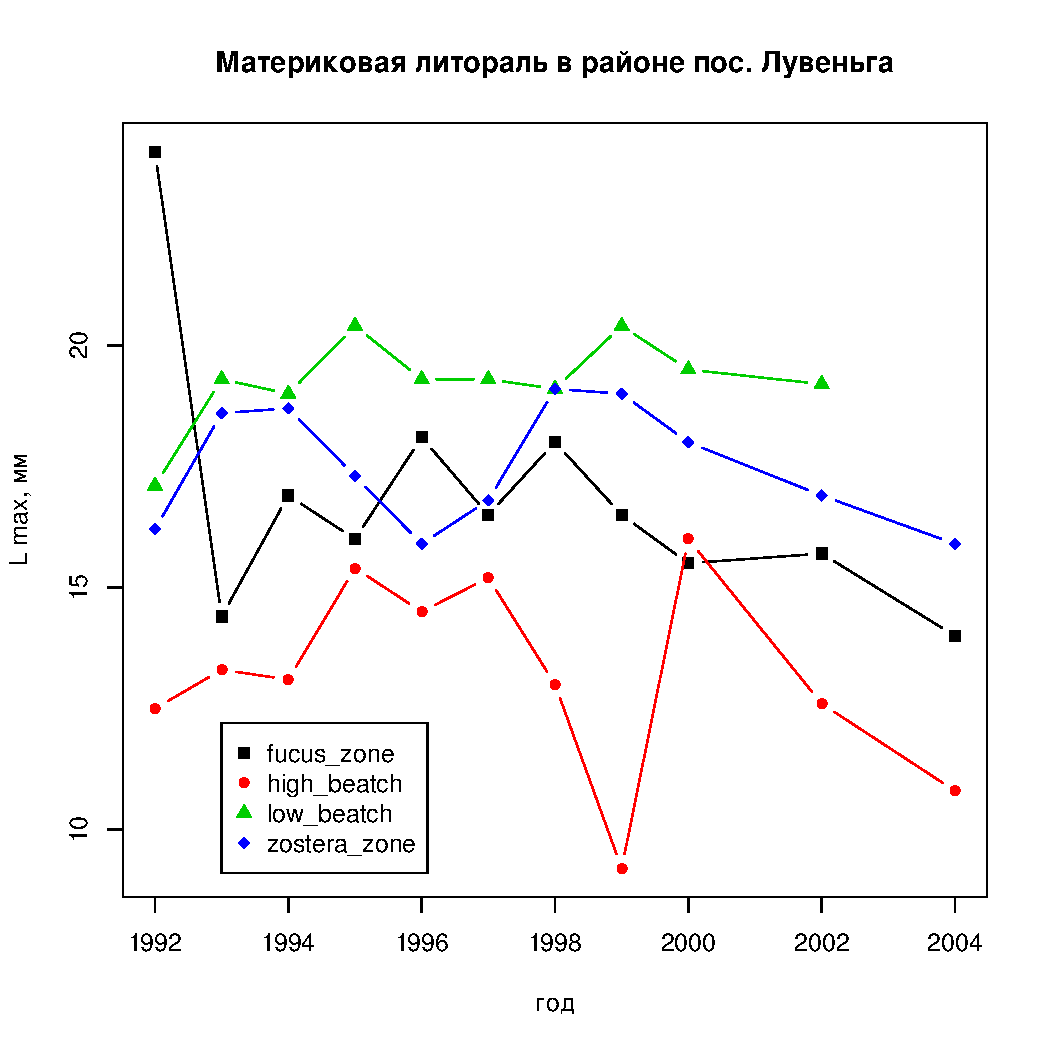
\includegraphics[width=65mm]{../White_Sea//Luvenga_II_razrez/L_max.pdf}
\end{center}
\end{minipage}

%\smallskip


\begin{minipage}[b]{.46\linewidth}
%Фигурка в первом ряду слева размер отведенный под весь этот объект -- 0.46 от ширины строки
%Параметр [b] означает, что выравнивание этих министраниц будет по нижнему краю
\begin{center}
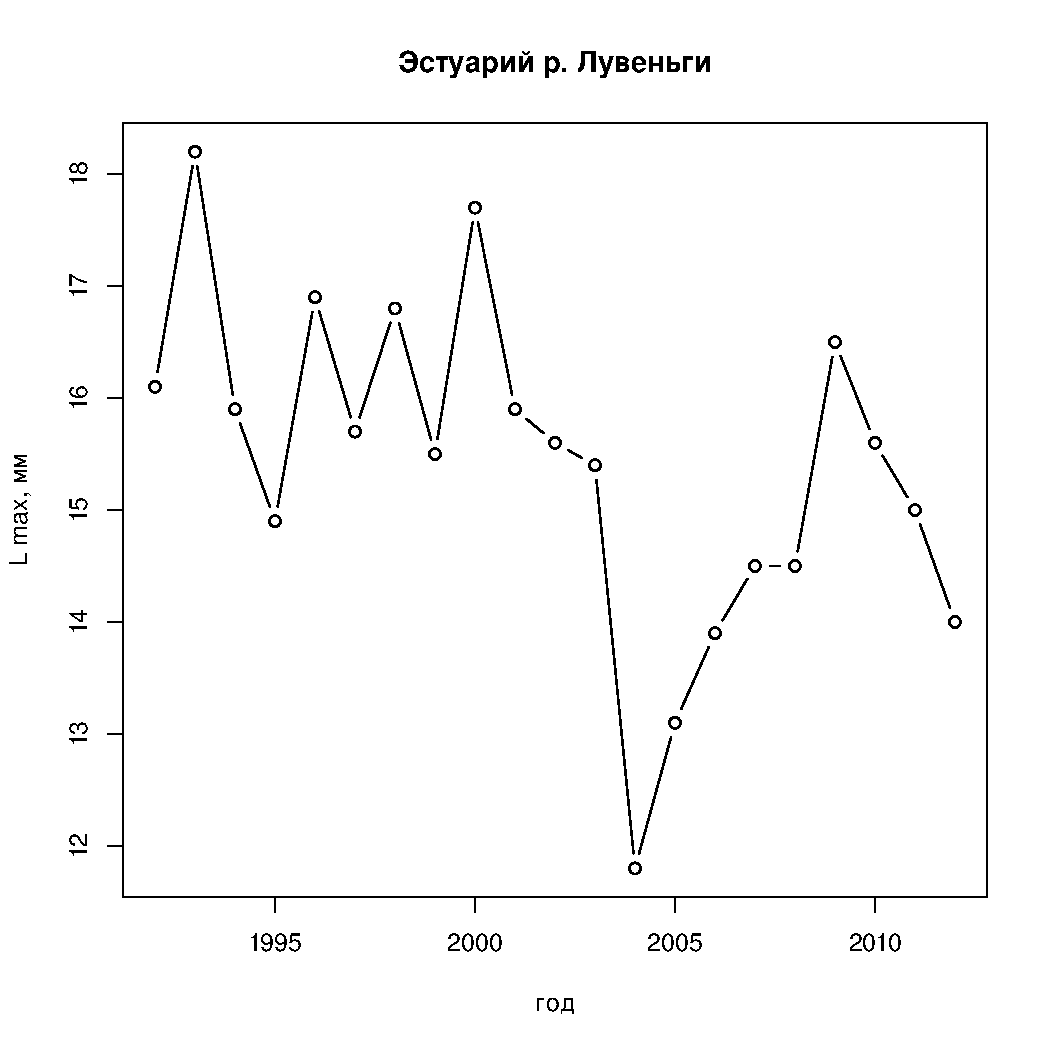
\includegraphics[width=65mm]{../White_Sea/Estuatiy_Luvenga/L_max.pdf}
\end{center}
\end{minipage}
%
\hfil %Это пружинка отодвигающая рисунки друг от друга
%
\begin{minipage}[b]{.46\linewidth}
%Следующий рисунок - первый ряд справа %DUNGEON S_4 \ AB
\begin{center}
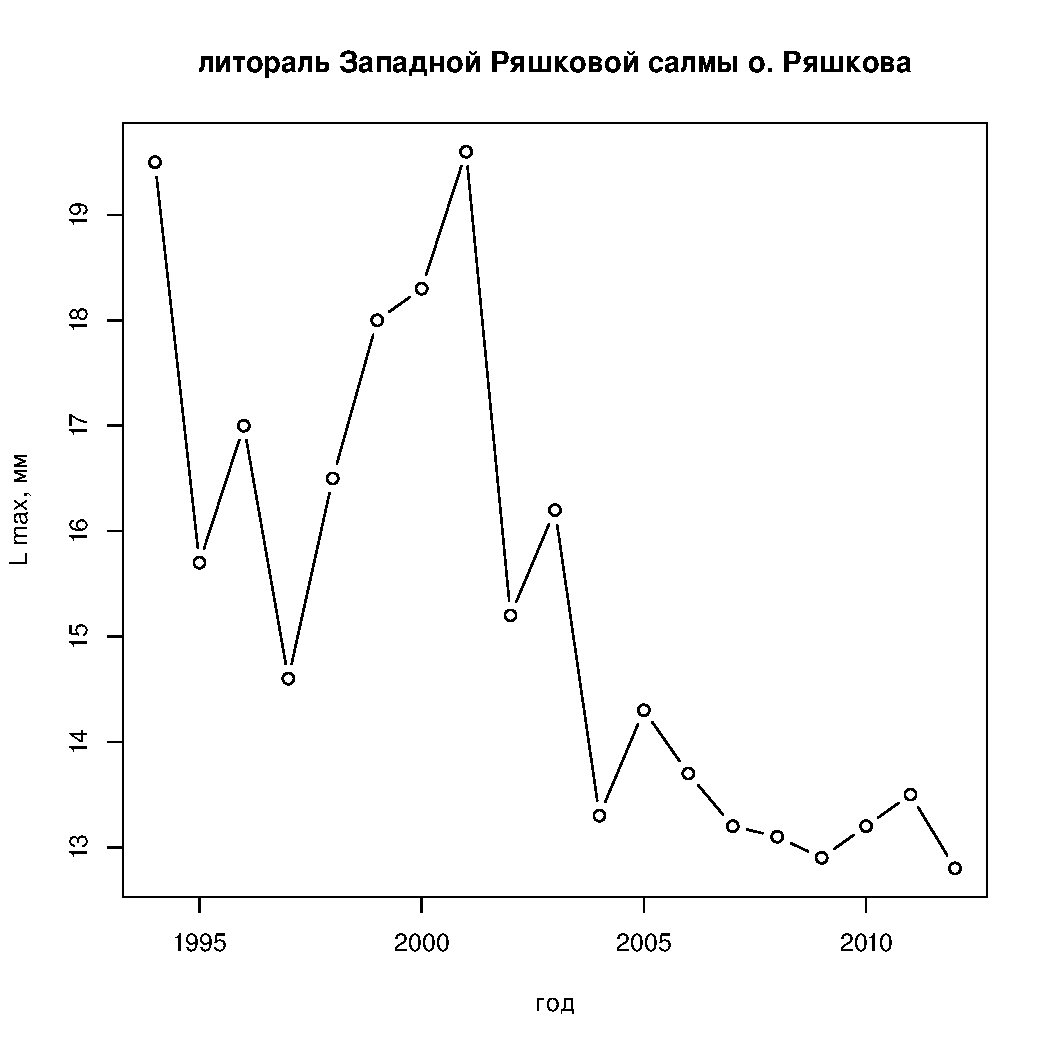
\includegraphics[width=65mm]{../White_Sea/Ryashkov_ZRS/L_max.pdf}
\end{center}
\end{minipage}

%\smallskip

\begin{minipage}[b]{.46\linewidth}
%Фигурка в первом ряду слева размер отведенный под весь этот объект -- 0.46 от ширины строки
%Параметр [b] означает, что выравнивание этих министраниц будет по нижнему краю
\begin{center}
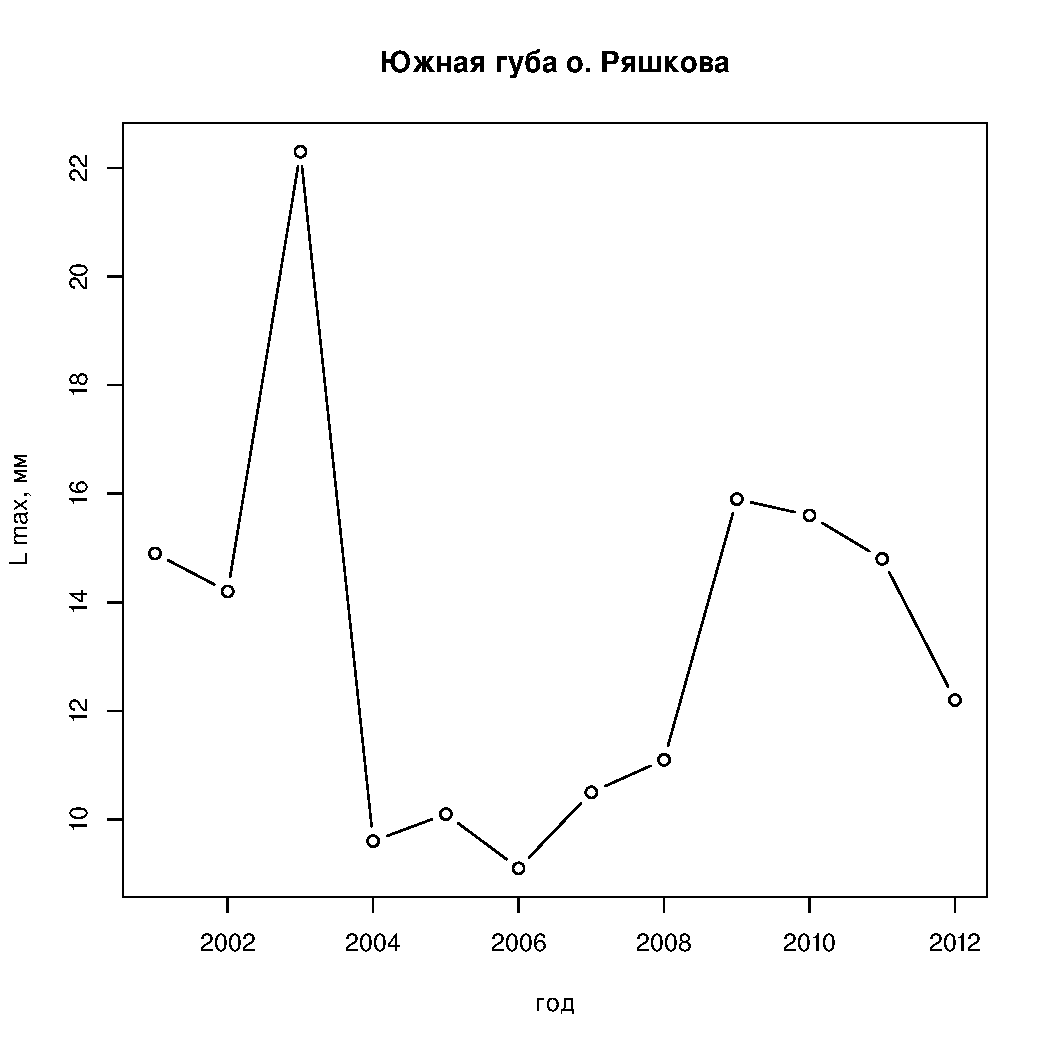
\includegraphics[width=65mm]{../White_Sea/Ryashkov_YuG/L_max.pdf}
\end{center}
\end{minipage}
%
\hfil %Это пружинка отодвигающая рисунки друг от друга
%
\begin{minipage}[b]{.46\linewidth}
%Следующий рисунок - первый ряд справа %DUNGEON S_4 \ AB
\begin{center}
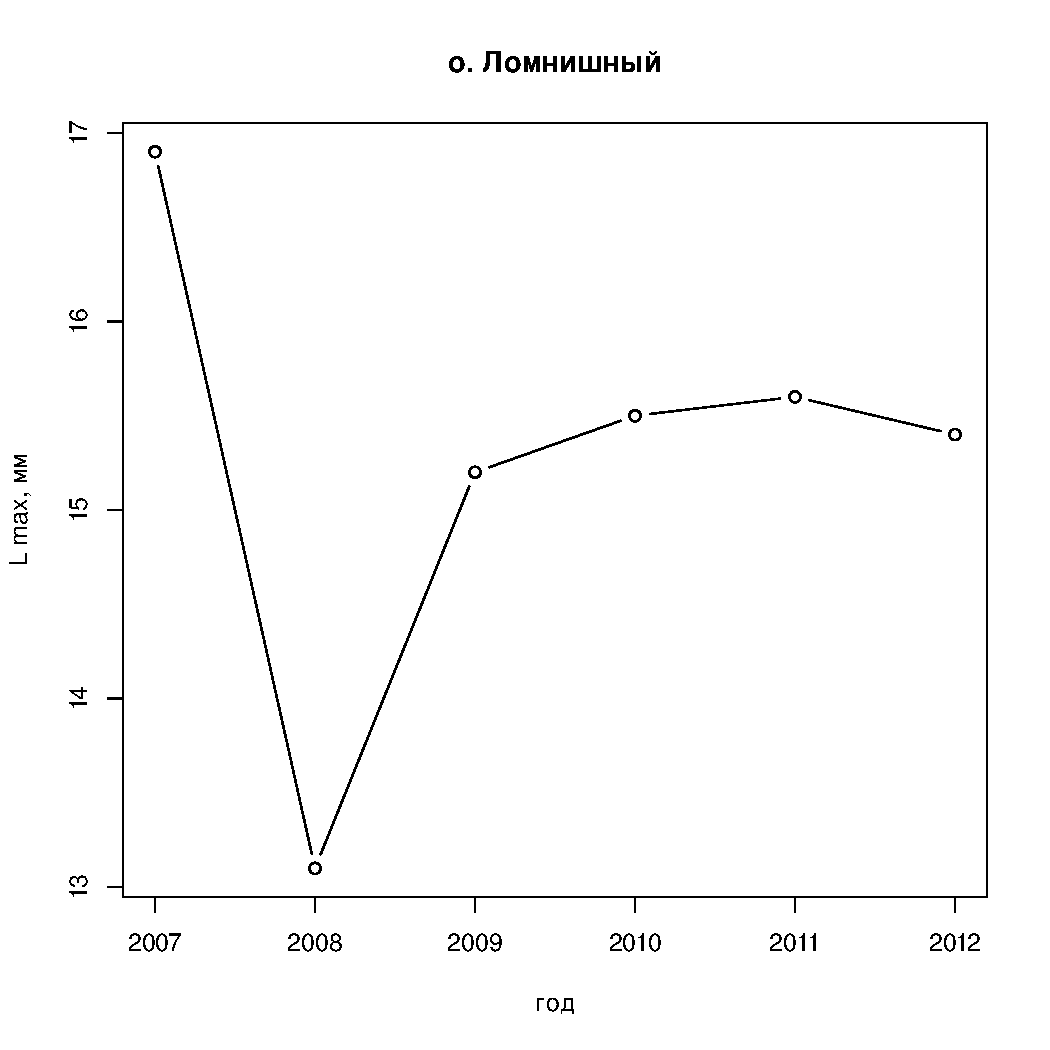
\includegraphics[width=65mm]{../White_Sea/Lomnishniy/L_max.pdf}
\end{center}
\end{minipage}

%\smallskip


\caption{Изменения максимальной длины особей {\it Macoma balthica} в исследованных поселениях}
\label{ris:Length_max}
\end{figure}

\subsection{Динамика биомассы}

\newpage
\begin{figure}[h]

\begin{minipage}[b]{.46\linewidth}
%Фигурка в первом ряду слева размер отведенный под весь этот объект -- 0.46 от ширины строки
%Параметр [b] означает, что выравнивание этих министраниц будет по нижнему краю
\begin{center}
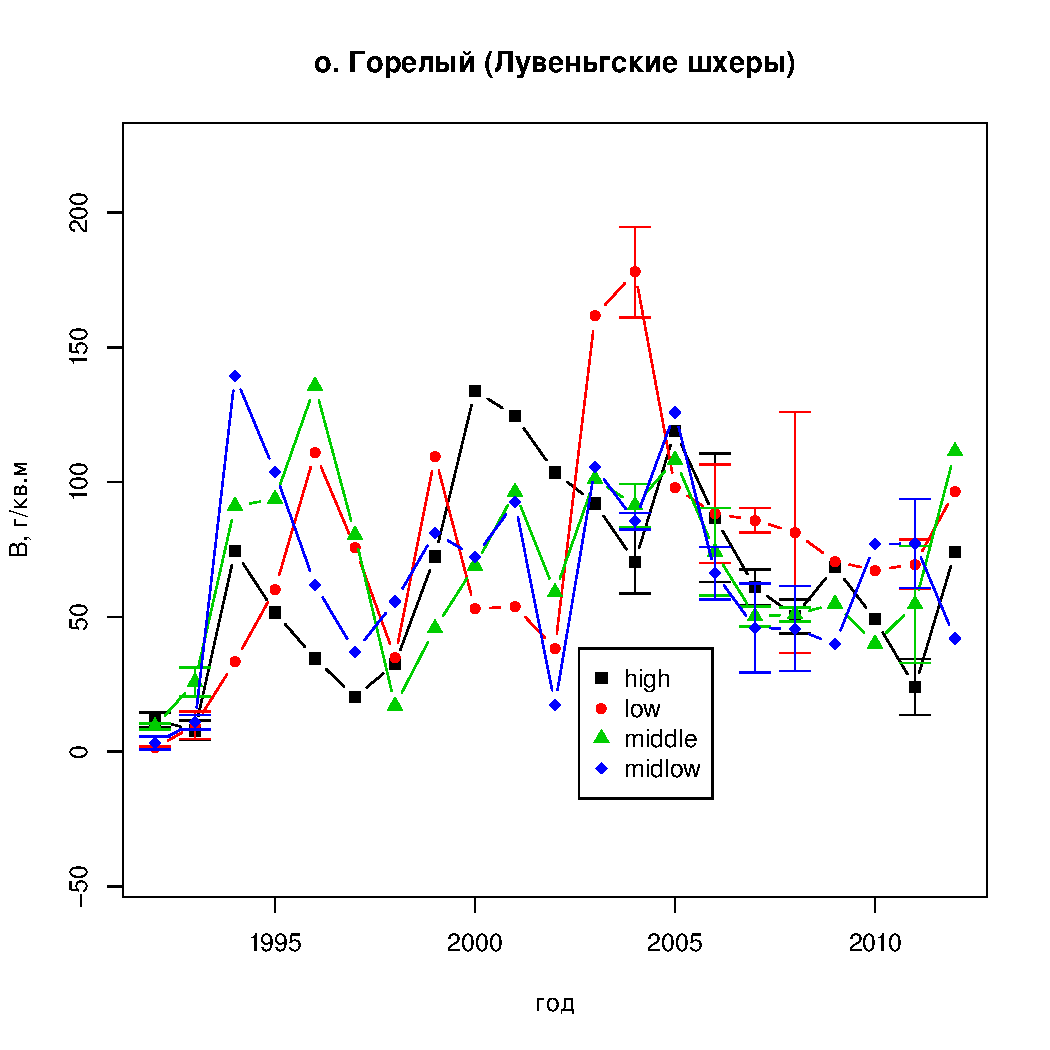
\includegraphics[width=65mm]{../White_Sea/Luvenga_Goreliy/B_count_dynamic.pdf}
\end{center}
\end{minipage}
%
\hfil %Это пружинка отодвигающая рисунки друг от друга
%
\begin{minipage}[b]{.46\linewidth}
%Следующий рисунок - первый ряд справа %DUNGEON S_4 \ AB
\begin{center}
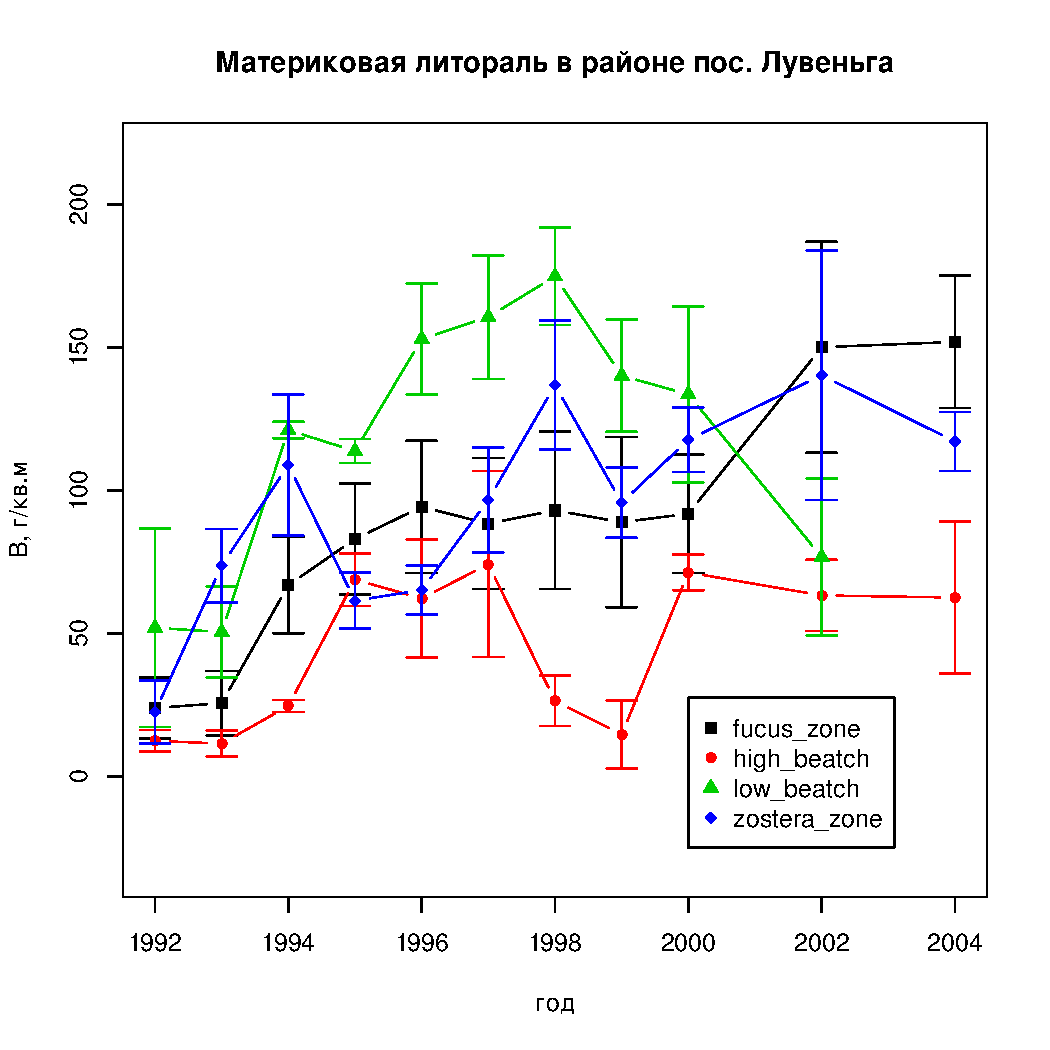
\includegraphics[width=65mm]{../White_Sea//Luvenga_II_razrez/B_count_dynamic.pdf}
\end{center}
\end{minipage}

%\smallskip


\begin{minipage}[b]{.46\linewidth}
%Фигурка в первом ряду слева размер отведенный под весь этот объект -- 0.46 от ширины строки
%Параметр [b] означает, что выравнивание этих министраниц будет по нижнему краю
\begin{center}
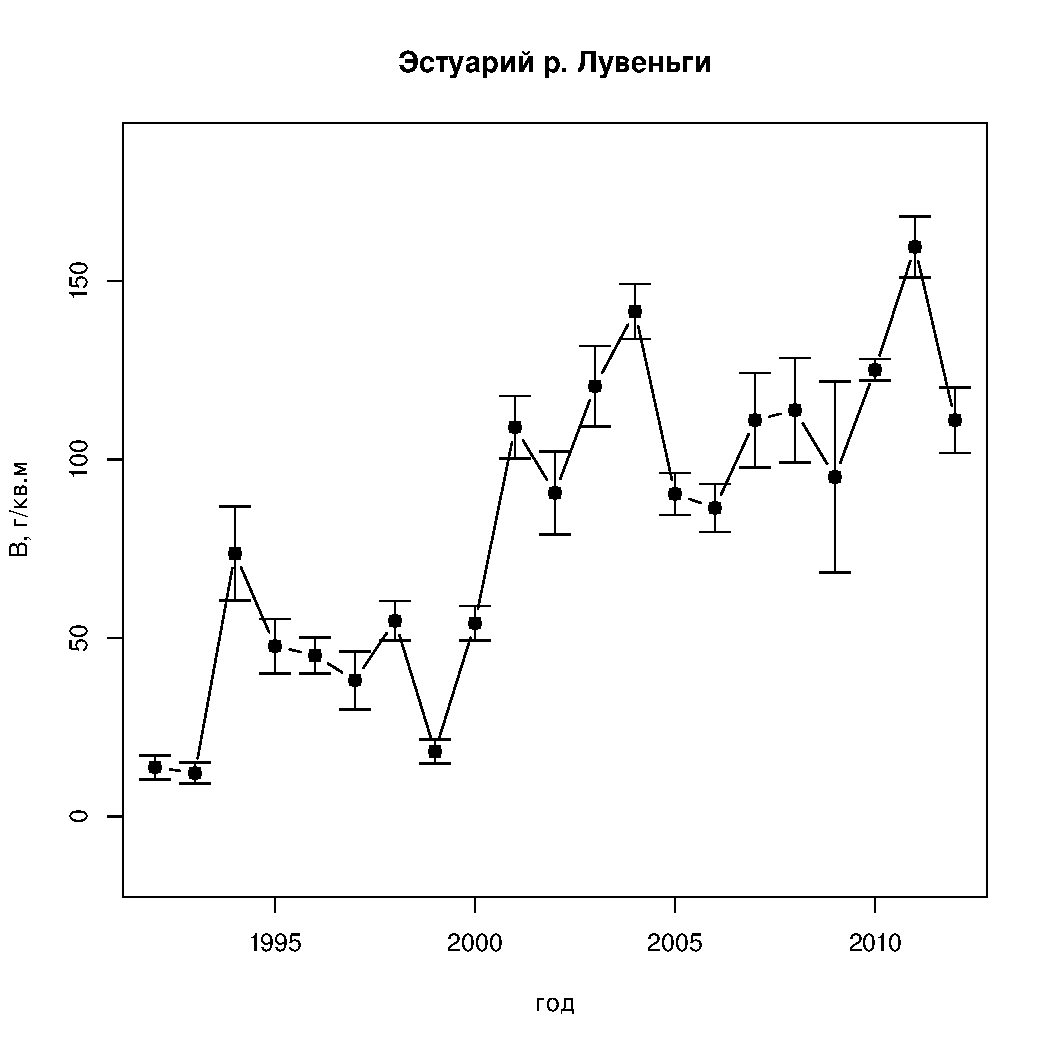
\includegraphics[width=65mm]{../White_Sea/Estuatiy_Luvenga/B_count_dynamic.pdf}
\end{center}
\end{minipage}
%
\hfil %Это пружинка отодвигающая рисунки друг от друга
%
\begin{minipage}[b]{.46\linewidth}
%Следующий рисунок - первый ряд справа %DUNGEON S_4 \ AB
\begin{center}
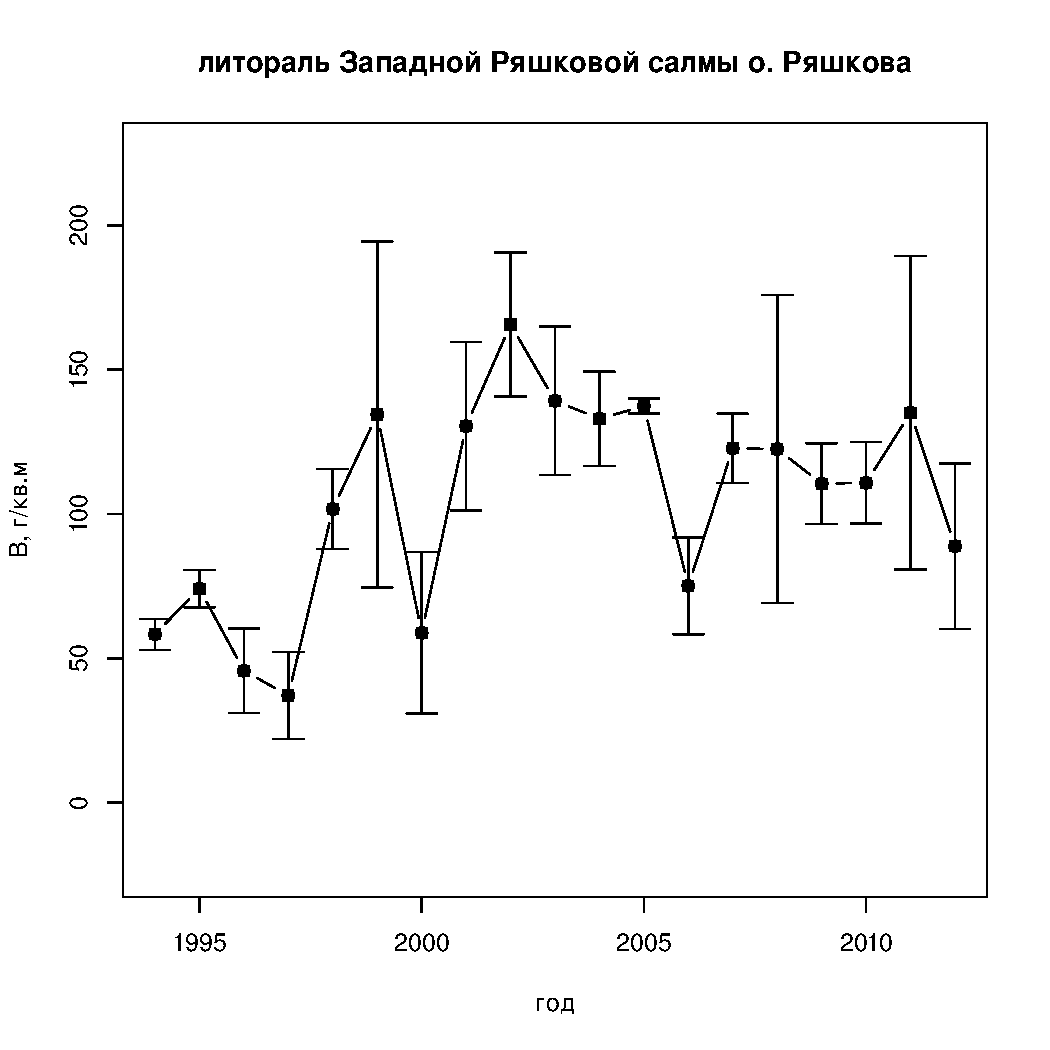
\includegraphics[width=65mm]{../White_Sea/Ryashkov_ZRS/B_count_dynamic.pdf}
\end{center}
\end{minipage}

%\smallskip

\begin{minipage}[b]{.46\linewidth}
%Фигурка в первом ряду слева размер отведенный под весь этот объект -- 0.46 от ширины строки
%Параметр [b] означает, что выравнивание этих министраниц будет по нижнему краю
\begin{center}
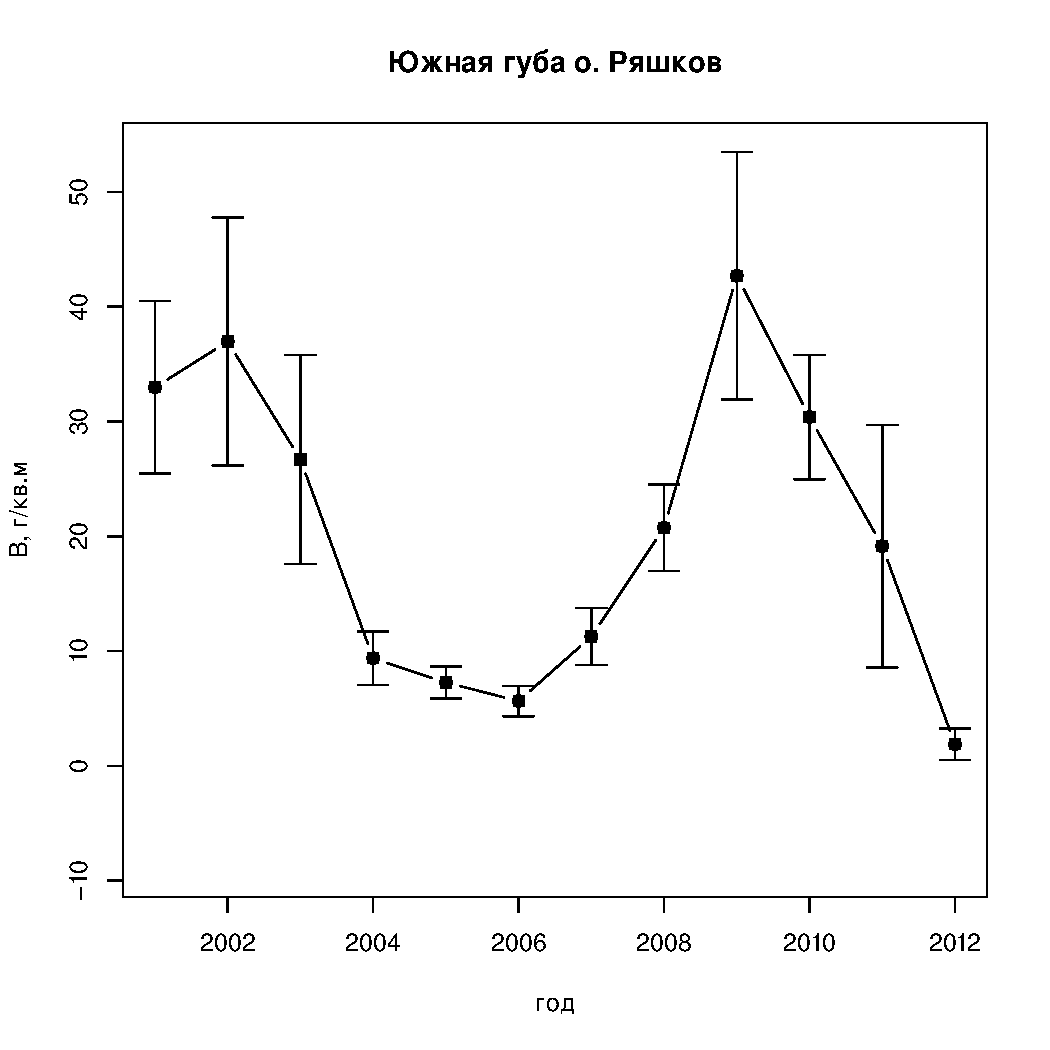
\includegraphics[width=65mm]{../White_Sea/Ryashkov_YuG/B_count_dynamic.pdf}
\end{center}
\end{minipage}
%
\hfil %Это пружинка отодвигающая рисунки друг от друга
%
\begin{minipage}[b]{.46\linewidth}
%Следующий рисунок - первый ряд справа %DUNGEON S_4 \ AB
\begin{center}
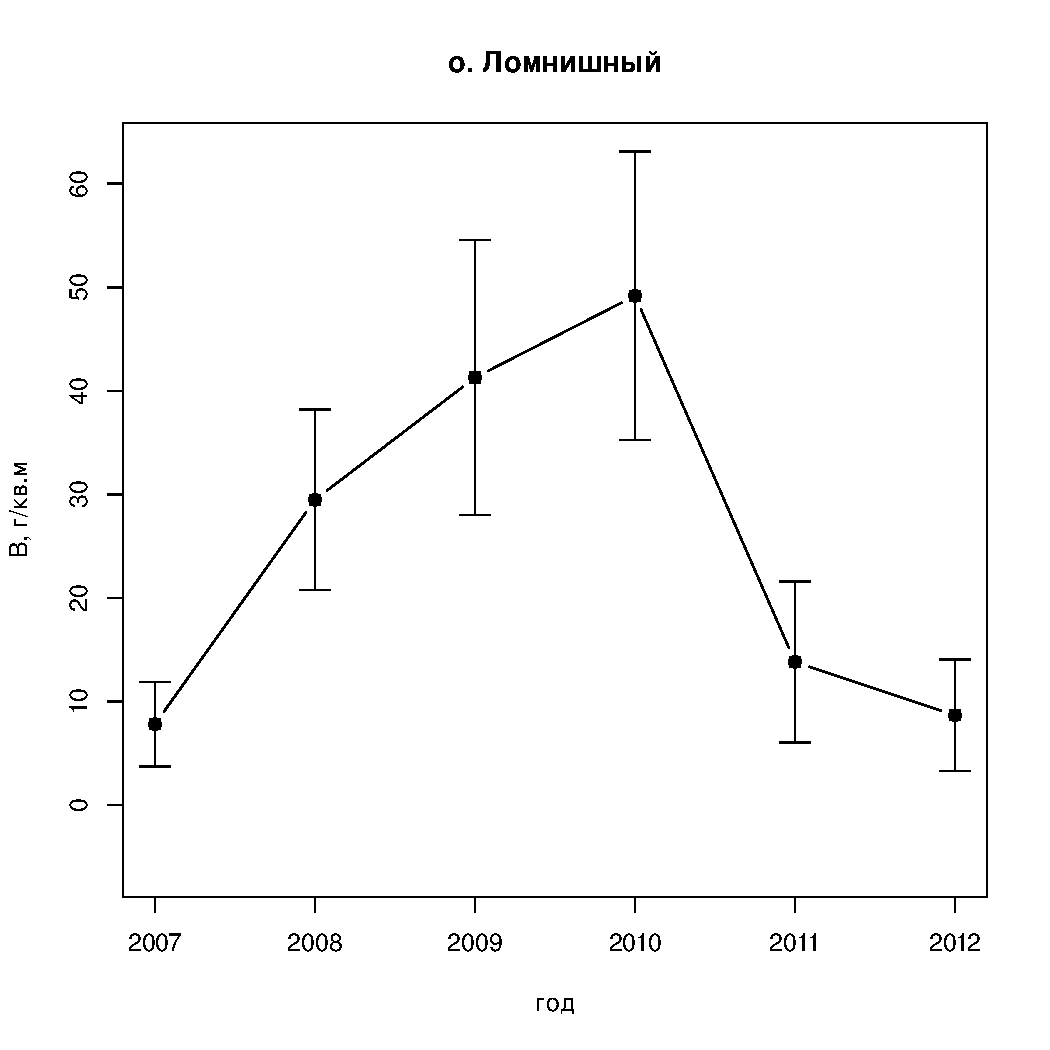
\includegraphics[width=65mm]{../White_Sea/Lomnishniy/B_count_dynamic.pdf}
\end{center}
\end{minipage}

%\smallskip


\caption{Динамика биомассы {\it Macoma balthica} в исследованных поселениях}
\label{ris:Length_max}
\end{figure}

        \section{Литература}
%        \bibliographystyle{rusnat}
        \bibliographystyle{gost780s}
%        \bibliographystyle{plain}
        \bibliography{/home/sonya/Dropbox/sophia_base}

\end{document}
